$\alpha = \beta = 1$ and $H = 0$.
Now we simulate our system for $t_f = 3, 5, 10, 15\sec$ and plot $K(t)$ matrix, $u(t)$ and states of system.

\begin{itemize}
	%%%%%%%%% tf = 3 %%%%%%%%%
	\item $t_f = 3\sec$
	\begin{figure}[H]
		\caption{$K(t)$ in $t_f = 3\sec$}
		\centering
		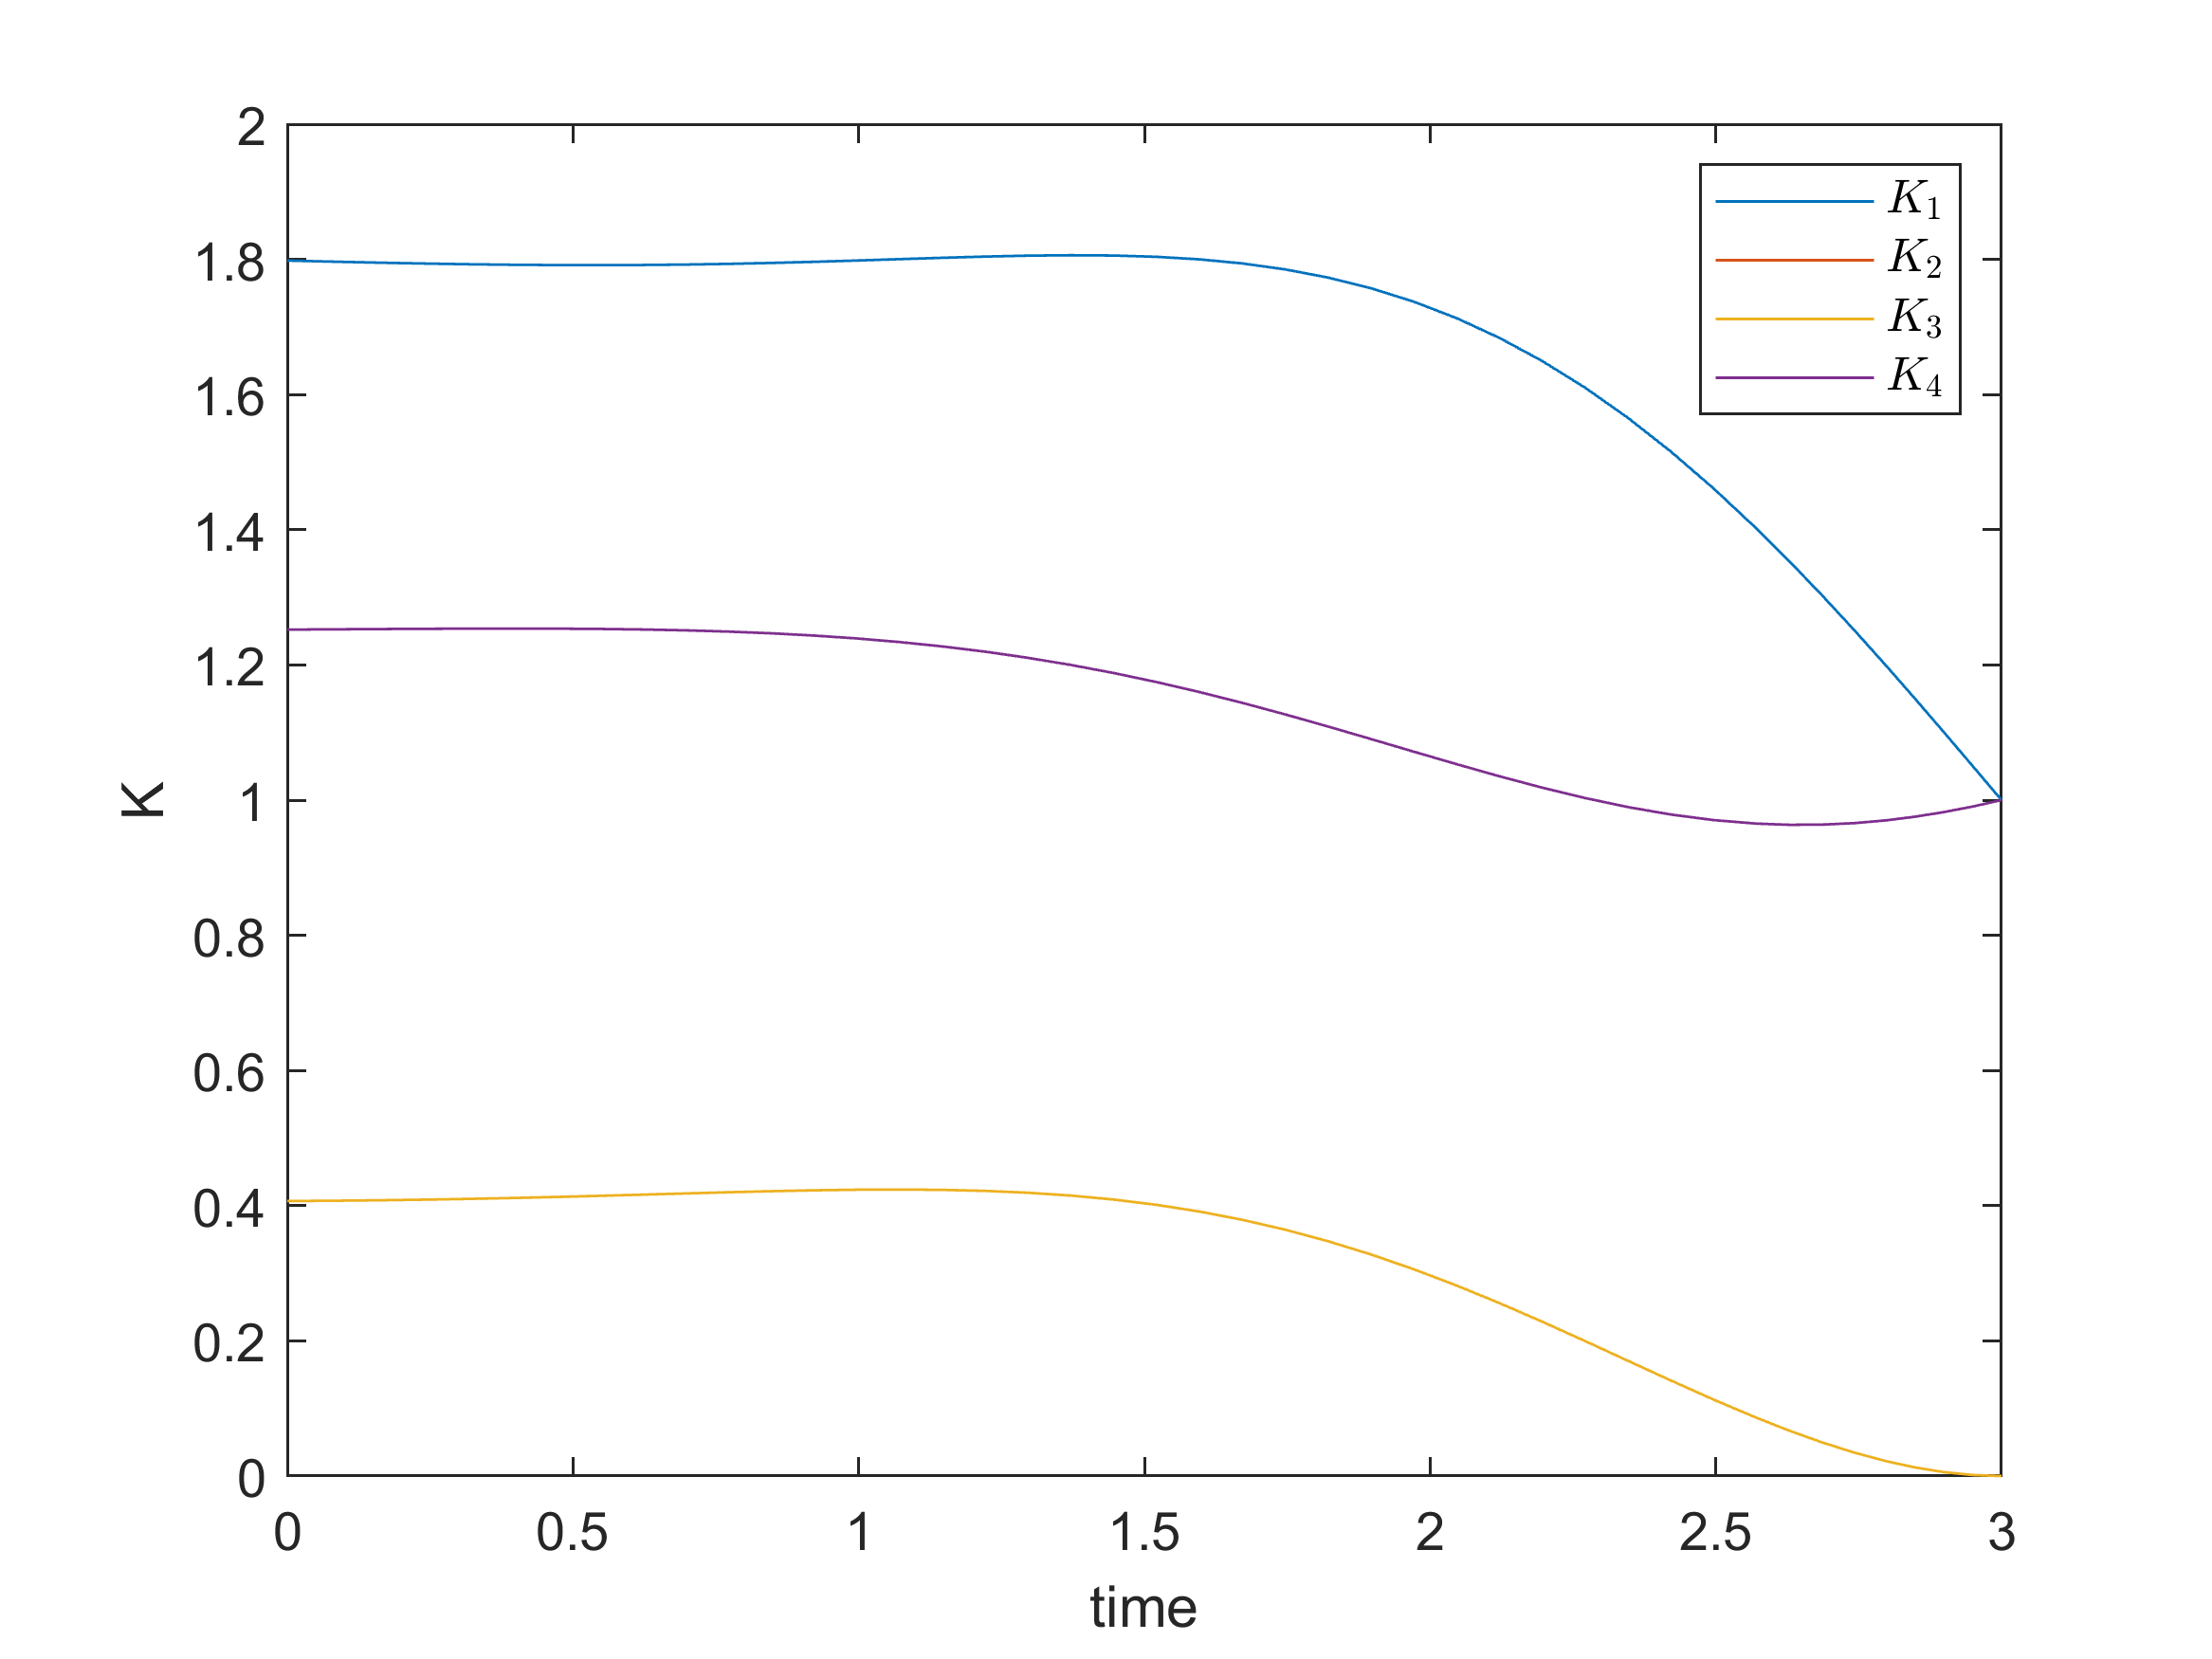
\includegraphics[width=12cm]{../Code/Q3/figures/K3.png}
	\end{figure}
\begin{figure}[H]
	\caption{$u(t)$ in $t_f = 3\sec$}
	\centering
	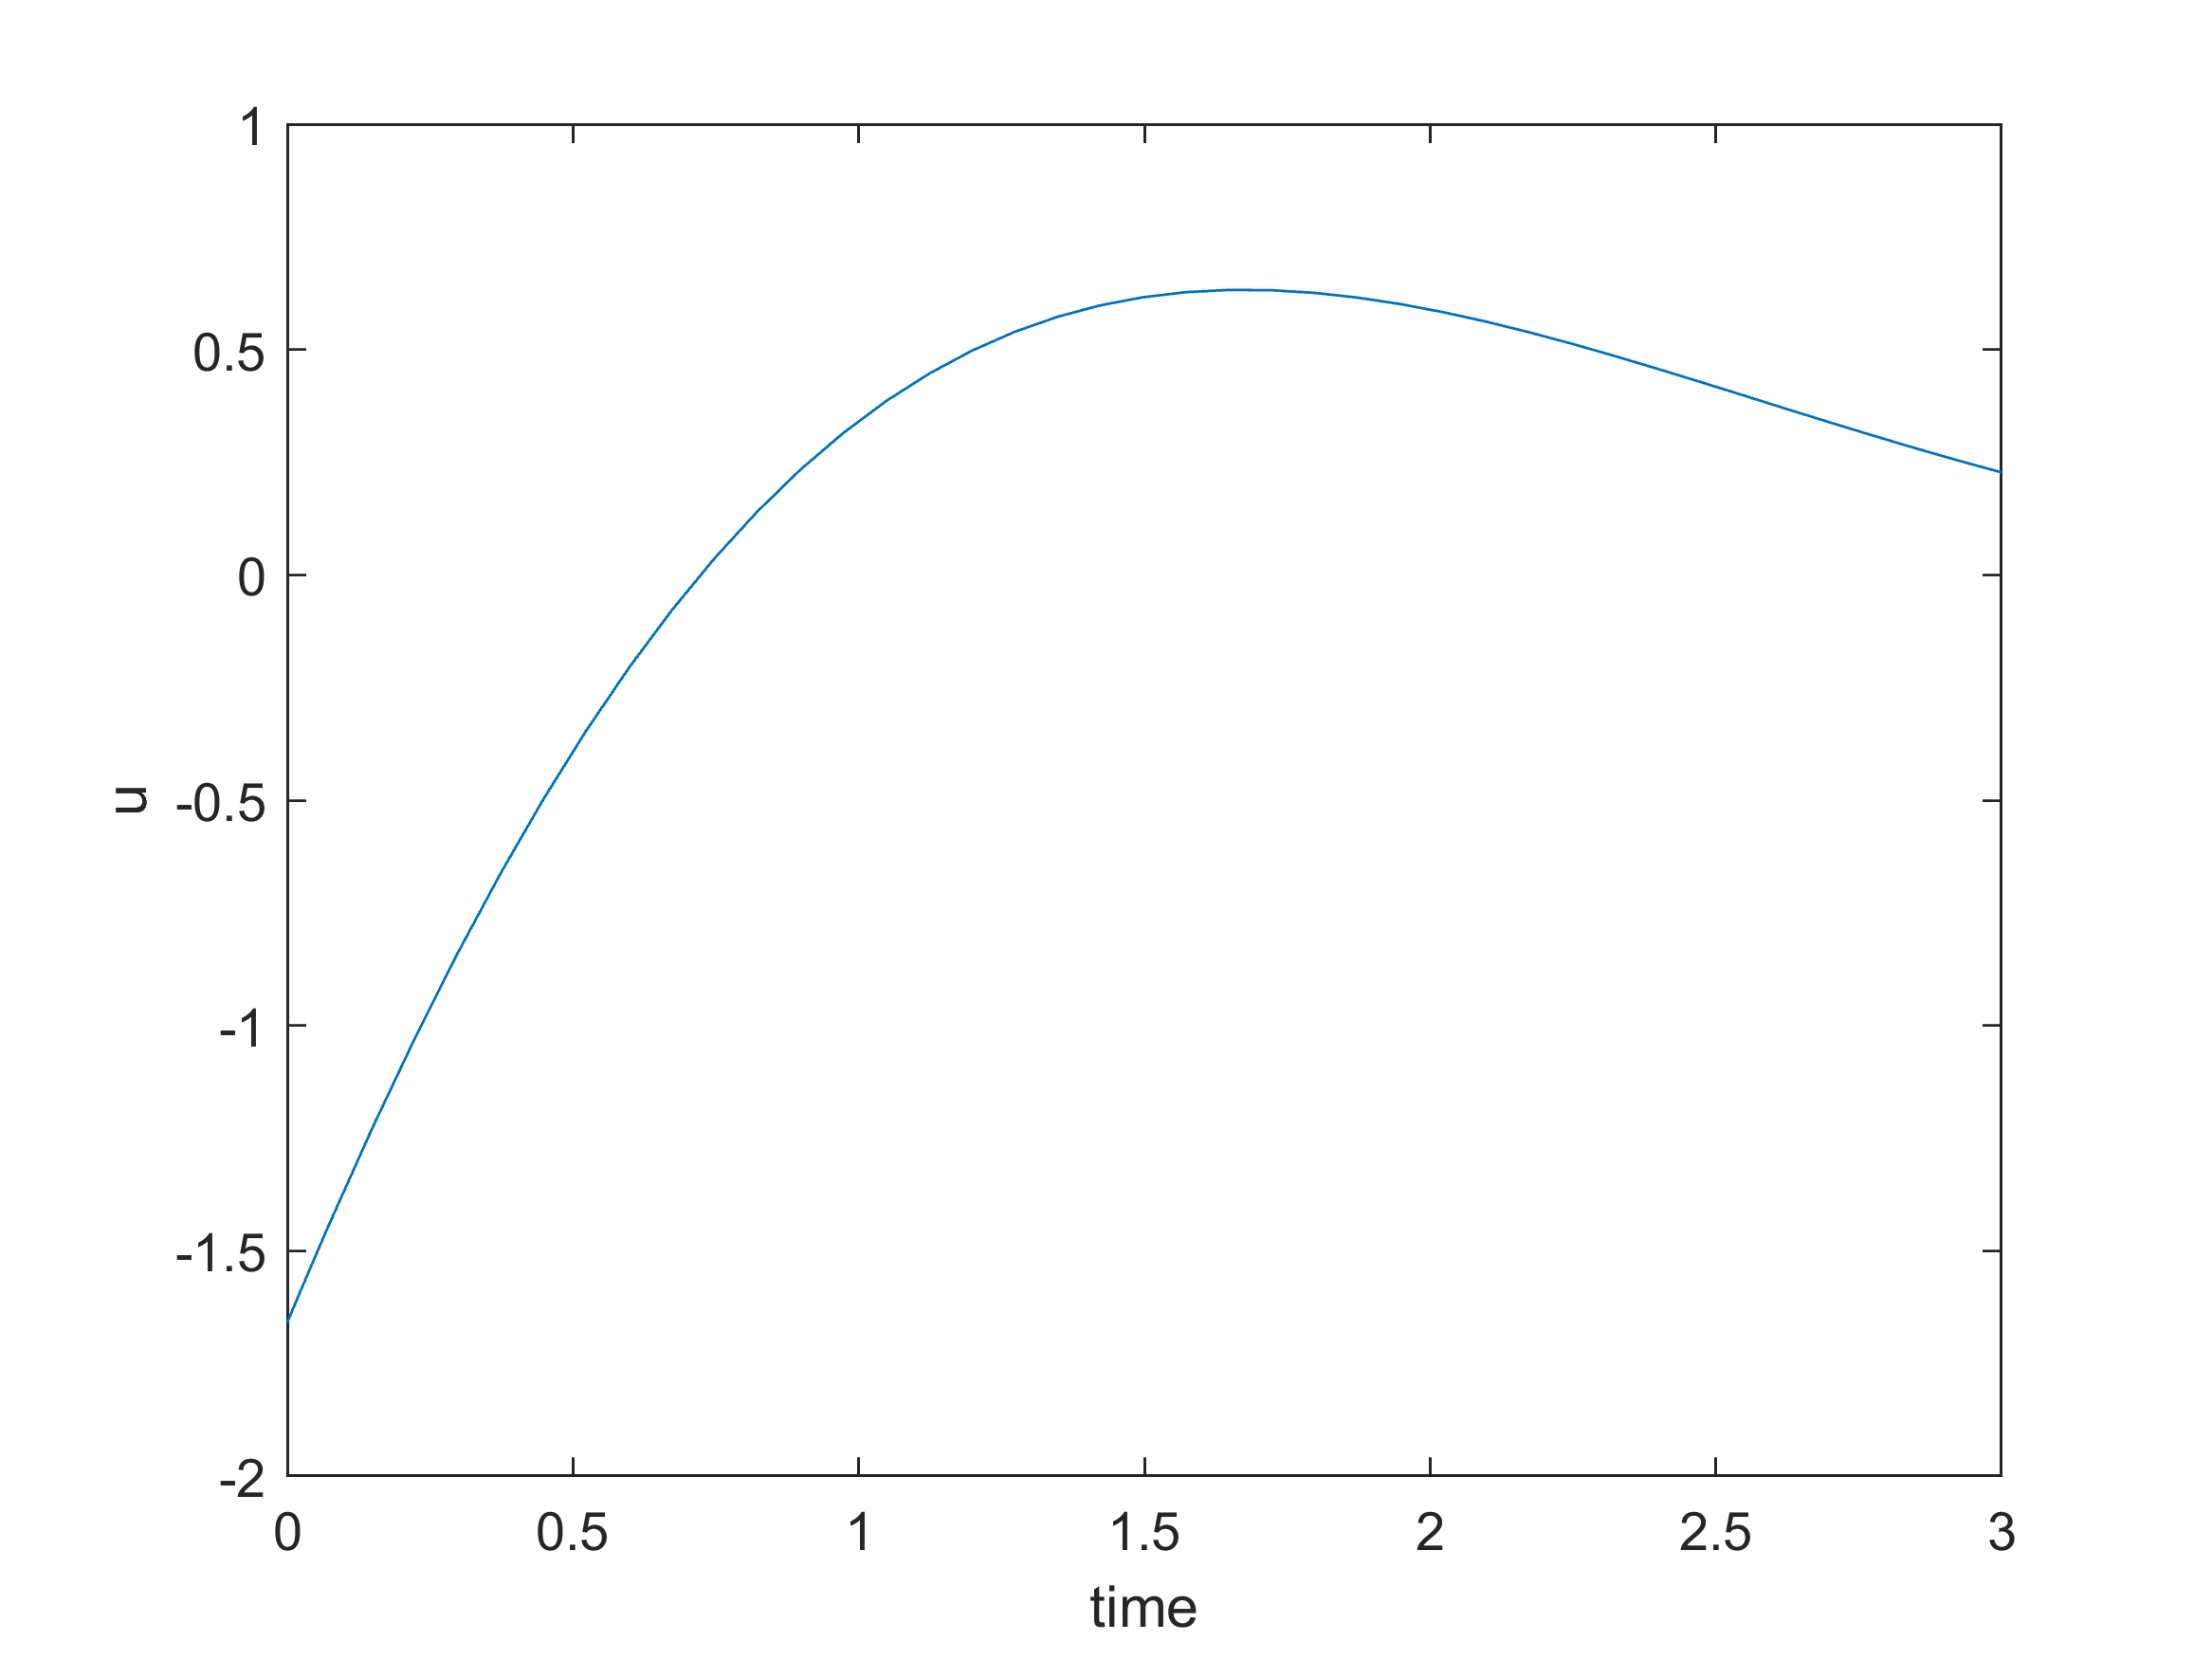
\includegraphics[width=12cm]{../Code/Q3/figures/u3.png}
\end{figure}
\begin{figure}[H]
	\caption{System States $\vec x(t)$ in $t_f = 3\sec$}
	\centering
	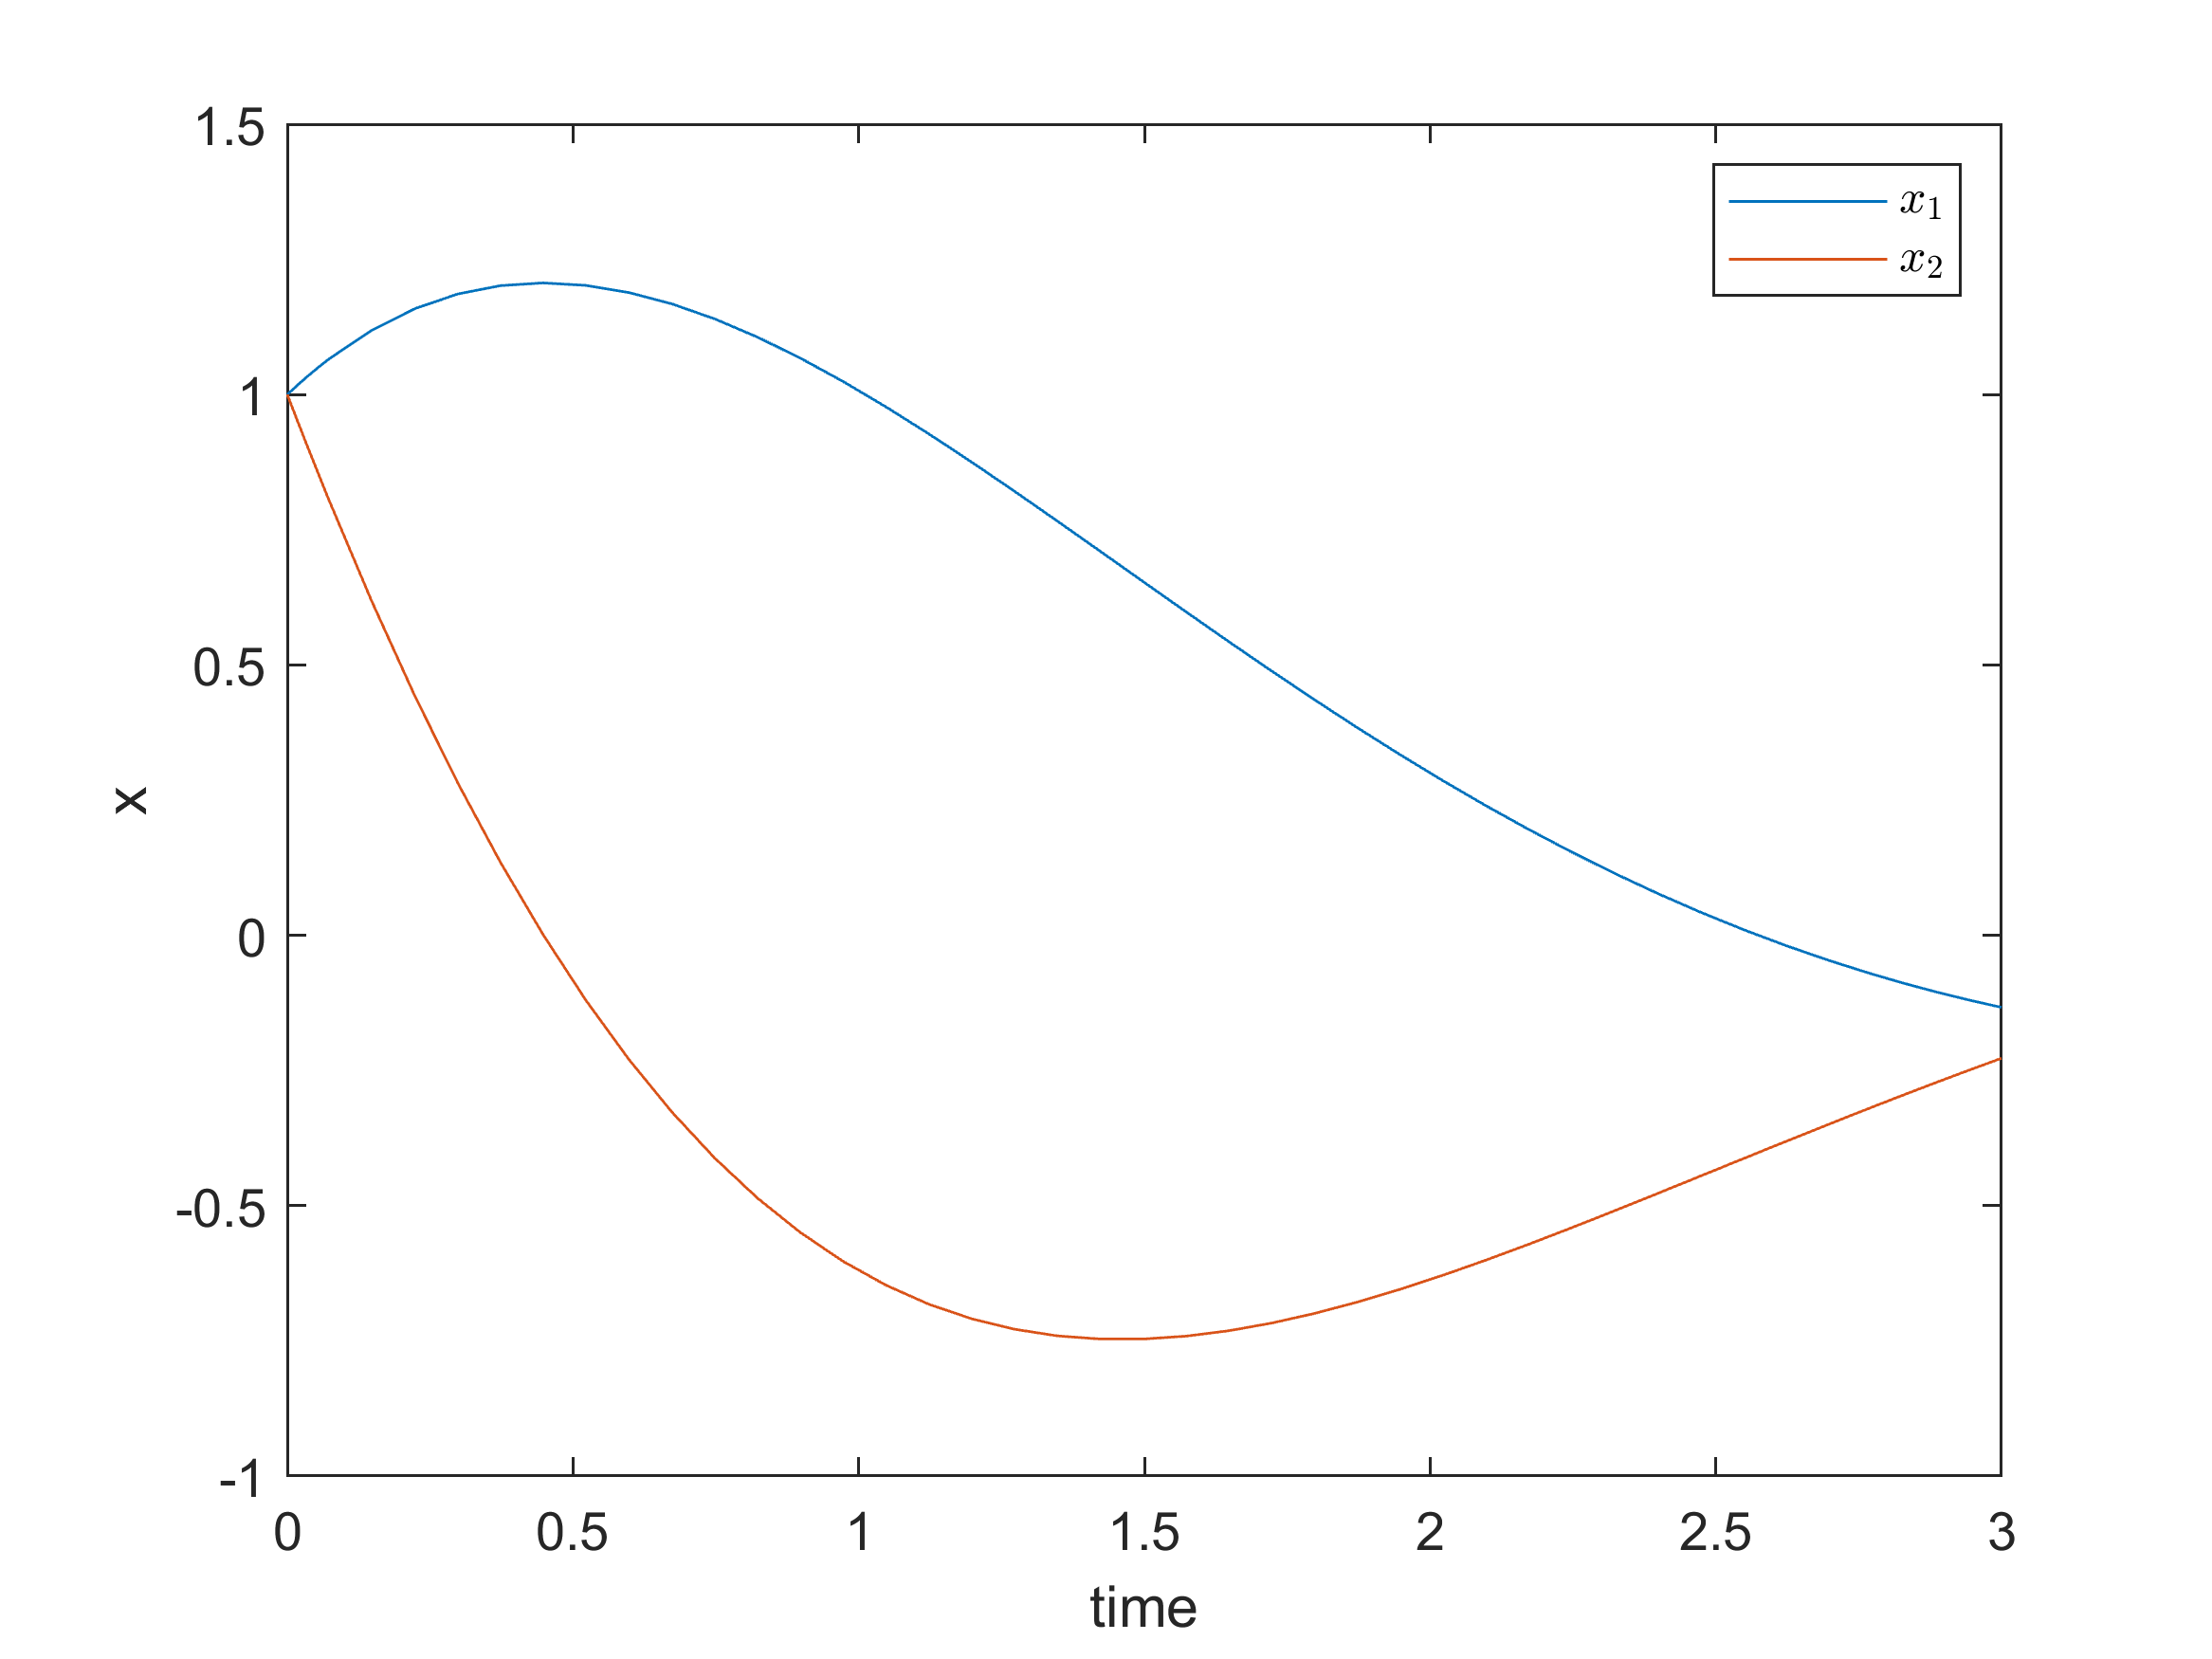
\includegraphics[width=12cm]{../Code/Q3/figures/tf3.png}
\end{figure}
%%%%%%%%% tf = 5 %%%%%%%%%
	\item $t_f = 5\sec$
	\begin{figure}[H]
		\caption{$K(t)$ in $t_f = 5\sec$}
		\centering
		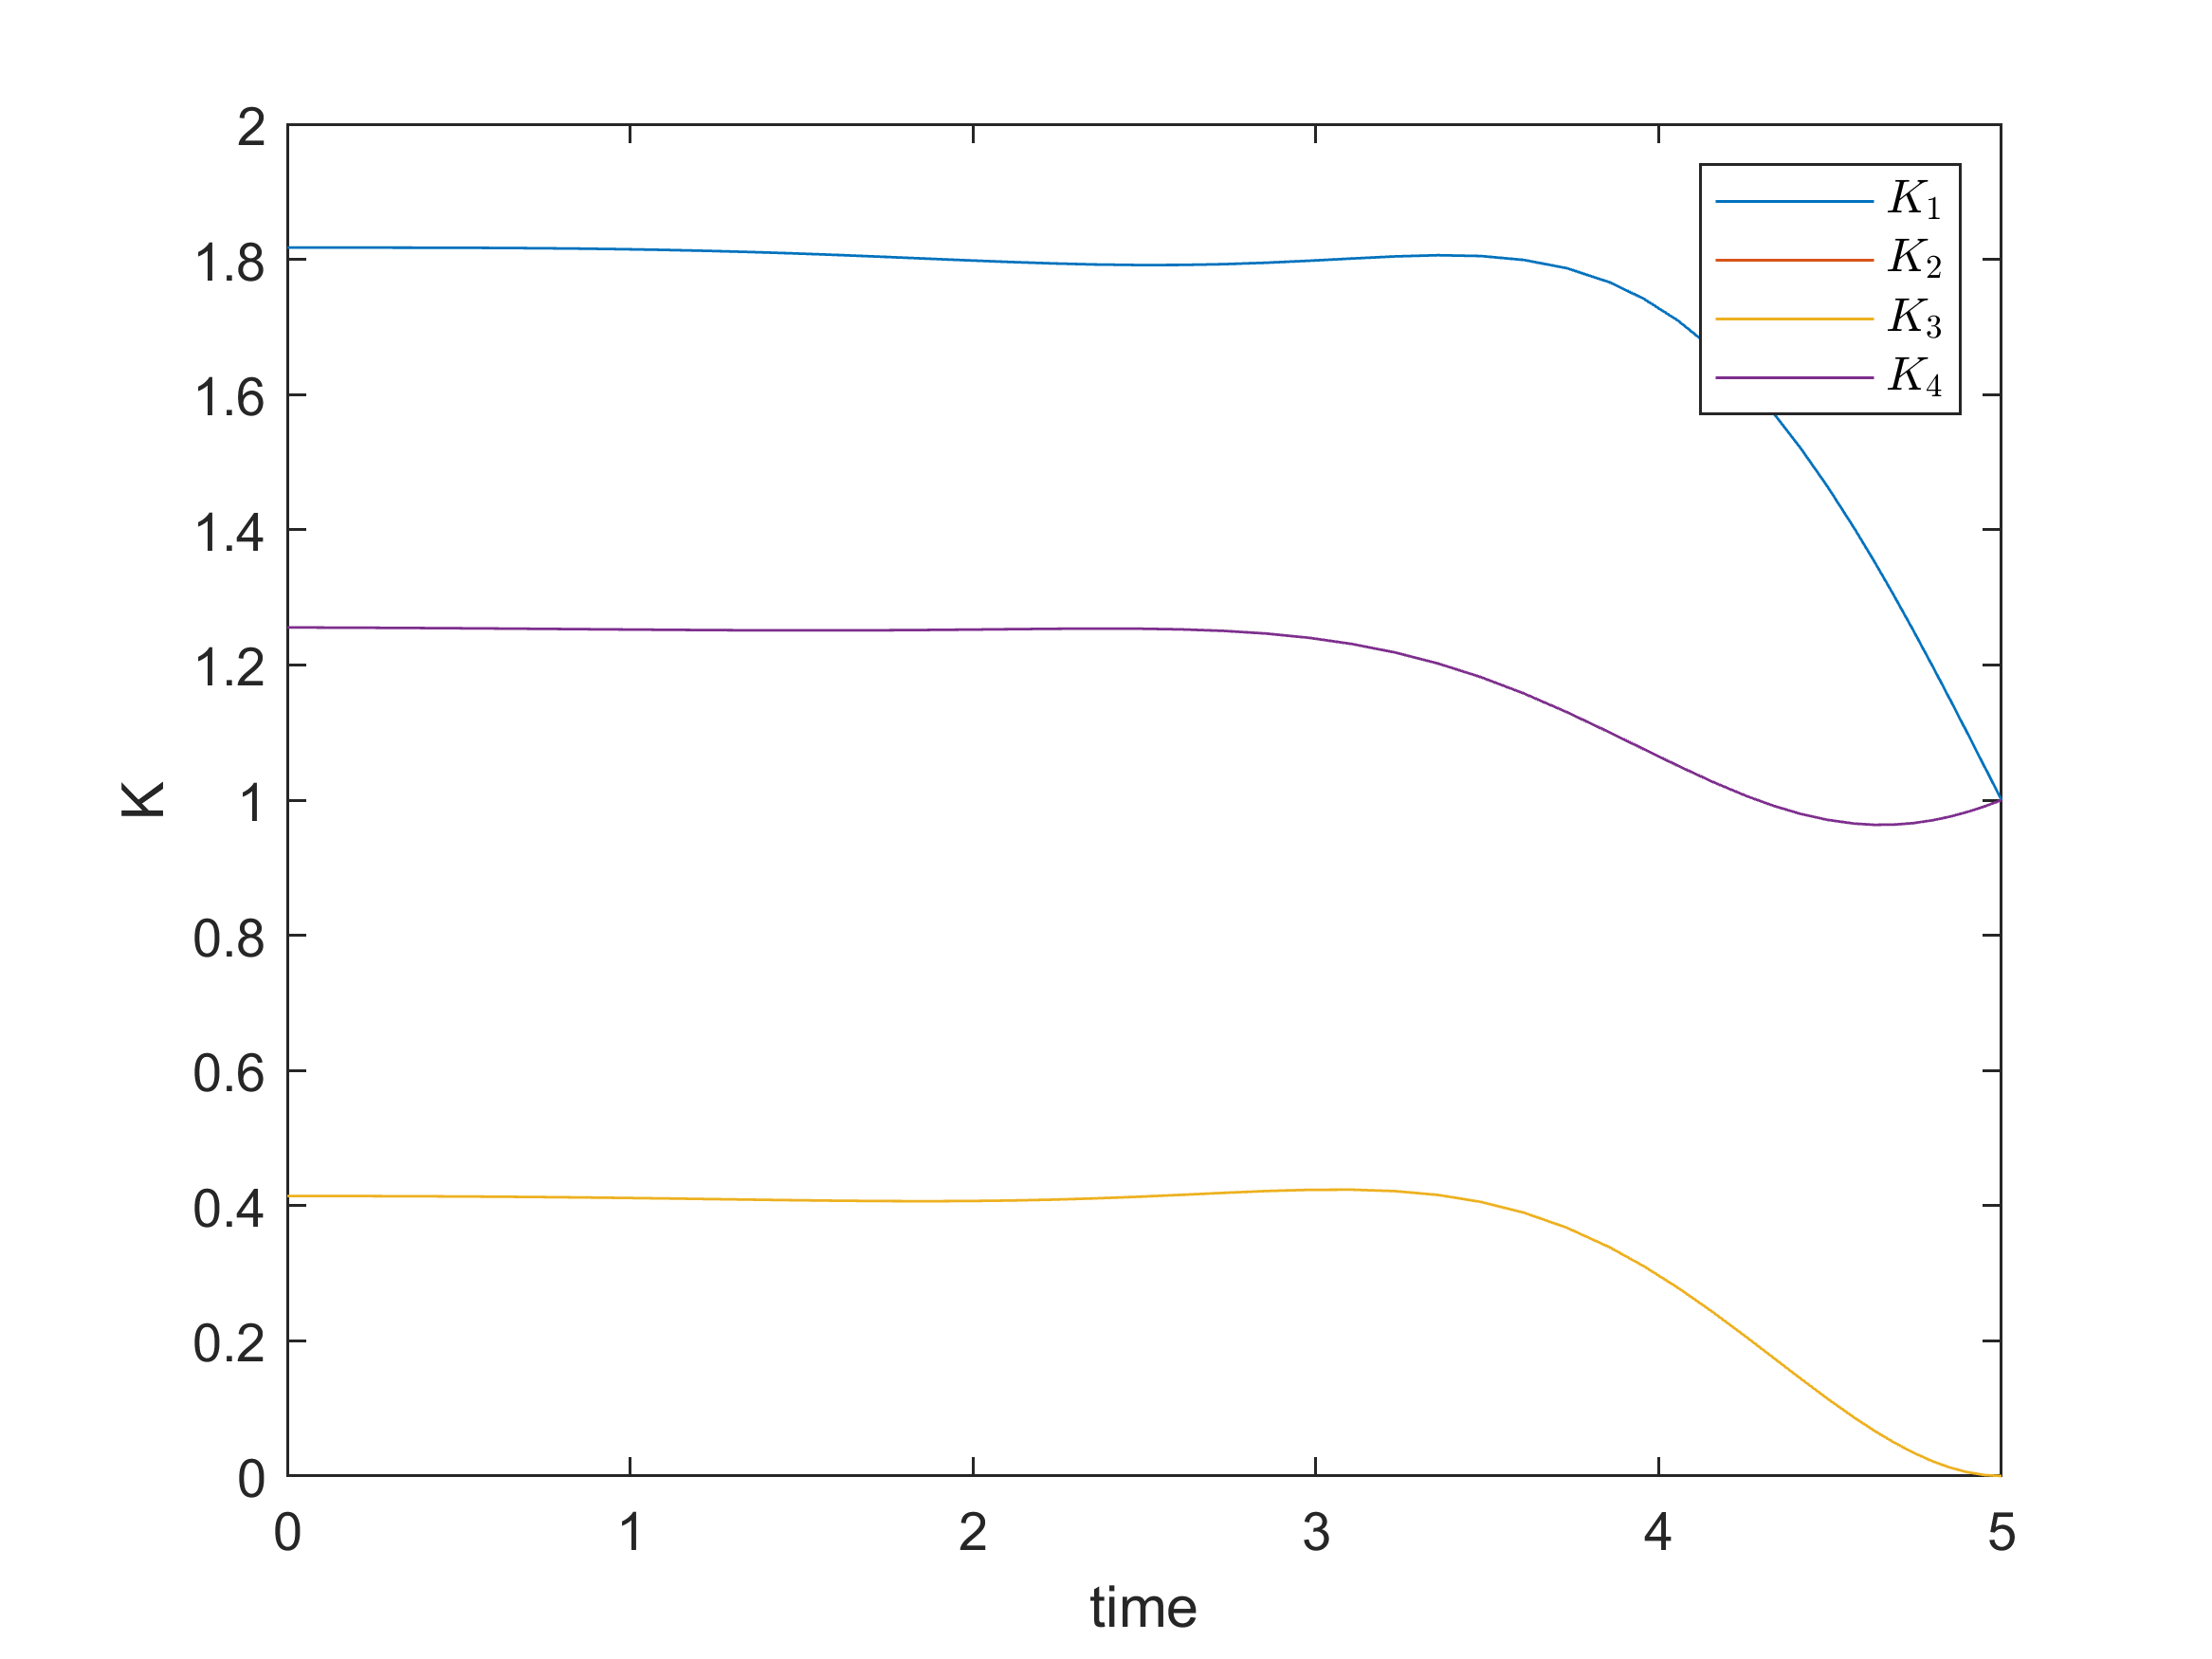
\includegraphics[width=12cm]{../Code/Q3/figures/K5.png}
	\end{figure}
	\begin{figure}[H]
		\caption{$u(t)$ in $t_f = 5\sec$}
		\centering
		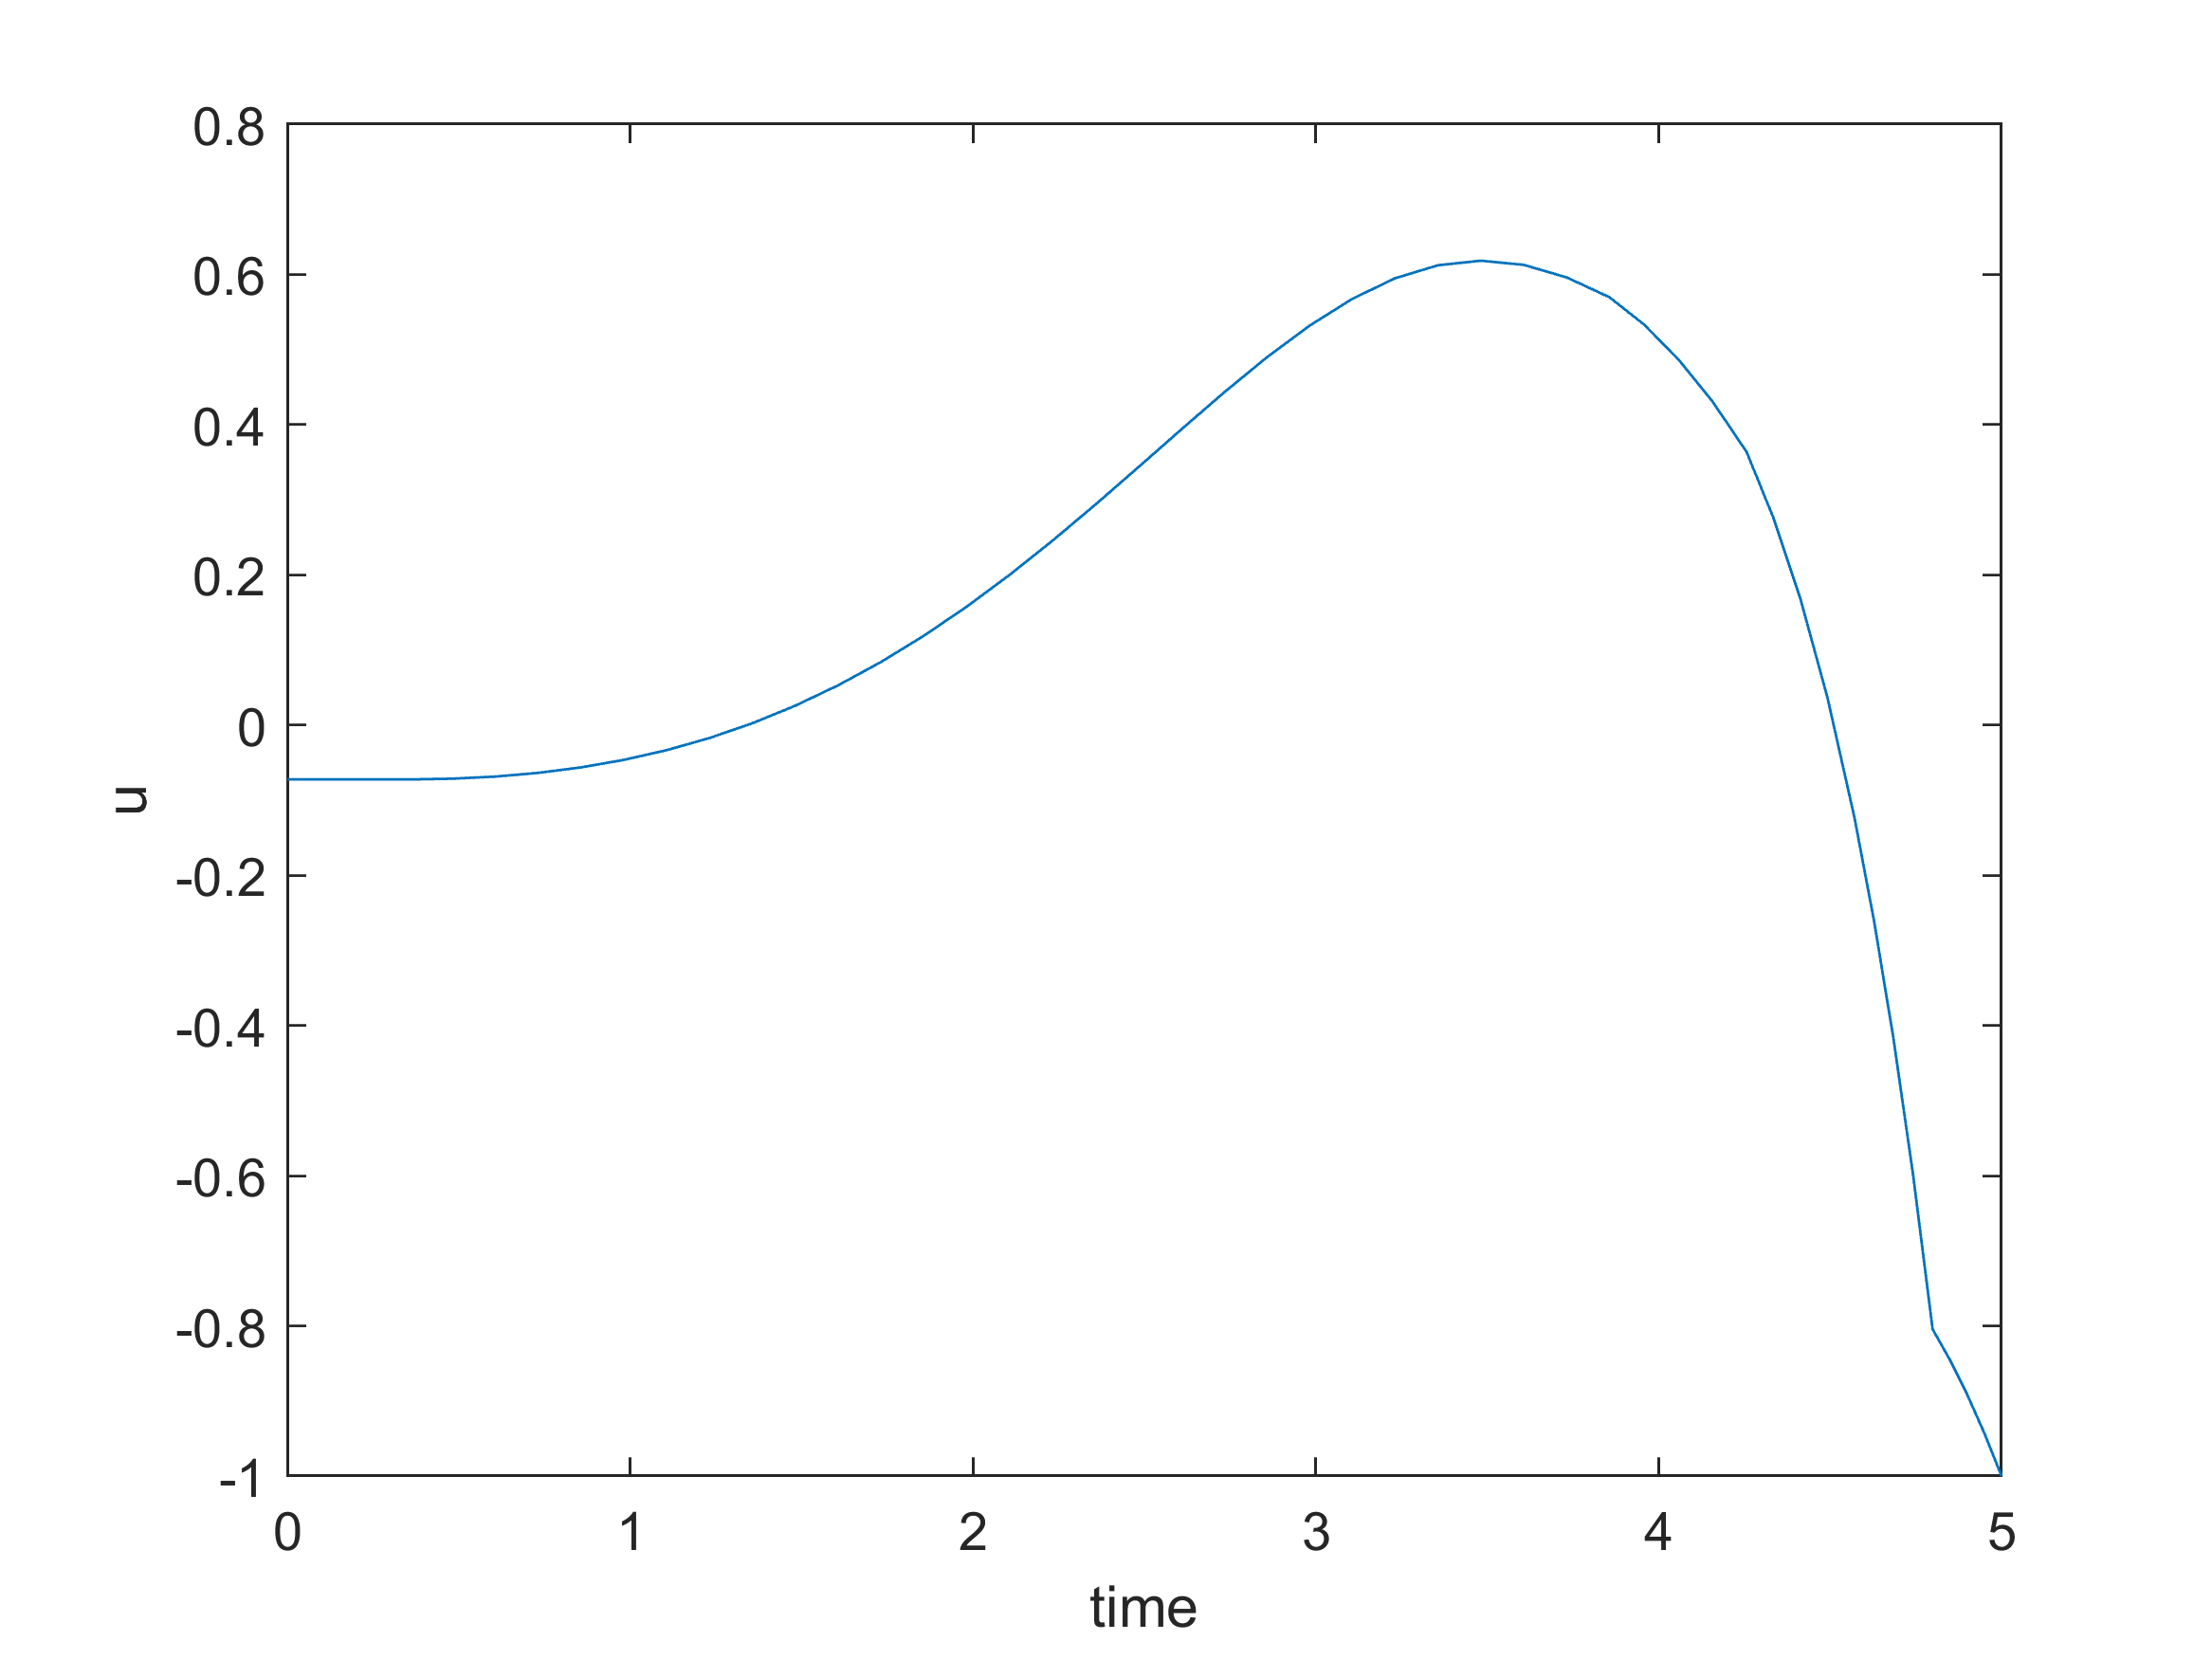
\includegraphics[width=12cm]{../Code/Q3/figures/u5.png}
	\end{figure}
	\begin{figure}[H]
		\caption{System States $\vec x(t)$ in $t_f = 5\sec$}
		\centering
		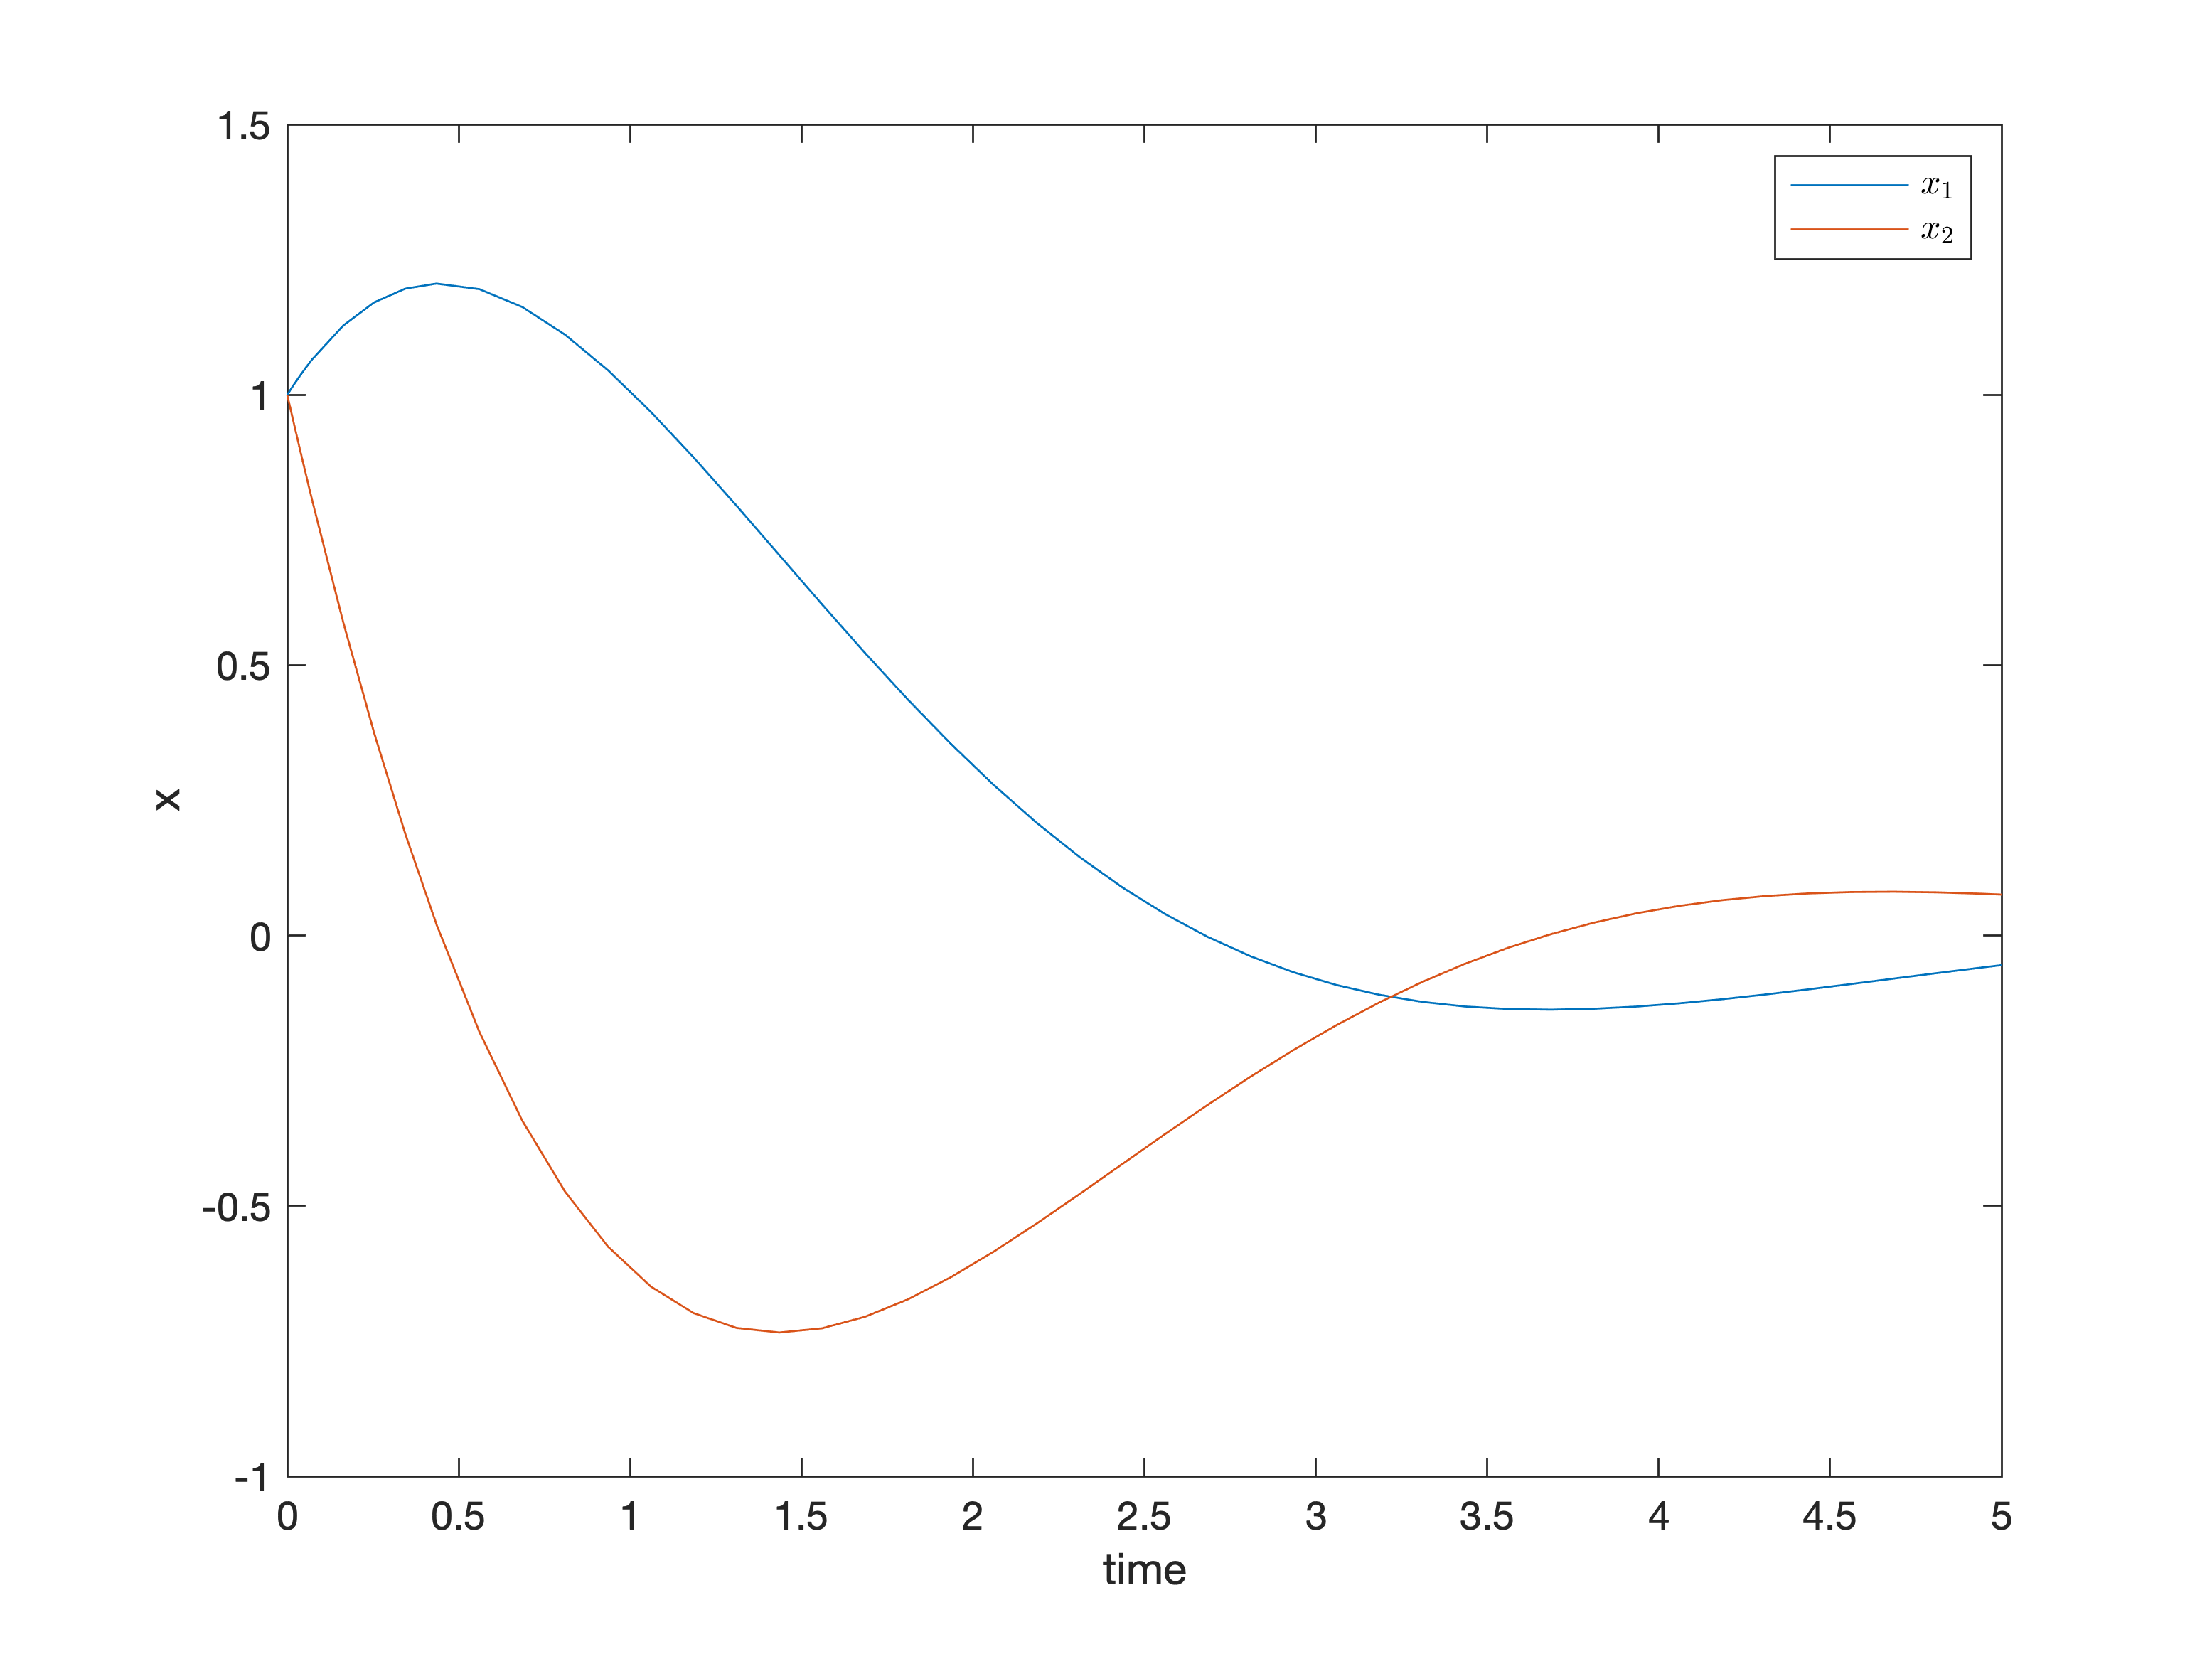
\includegraphics[width=12cm]{../Code/Q3/figures/tf5.png}
	\end{figure}
%%%%%%%%% tf = 10 %%%%%%%%%
\item $t_f = 10\sec$
\begin{figure}[H]
	\caption{$K(t)$ in $t_f = 10\sec$}
	\centering
	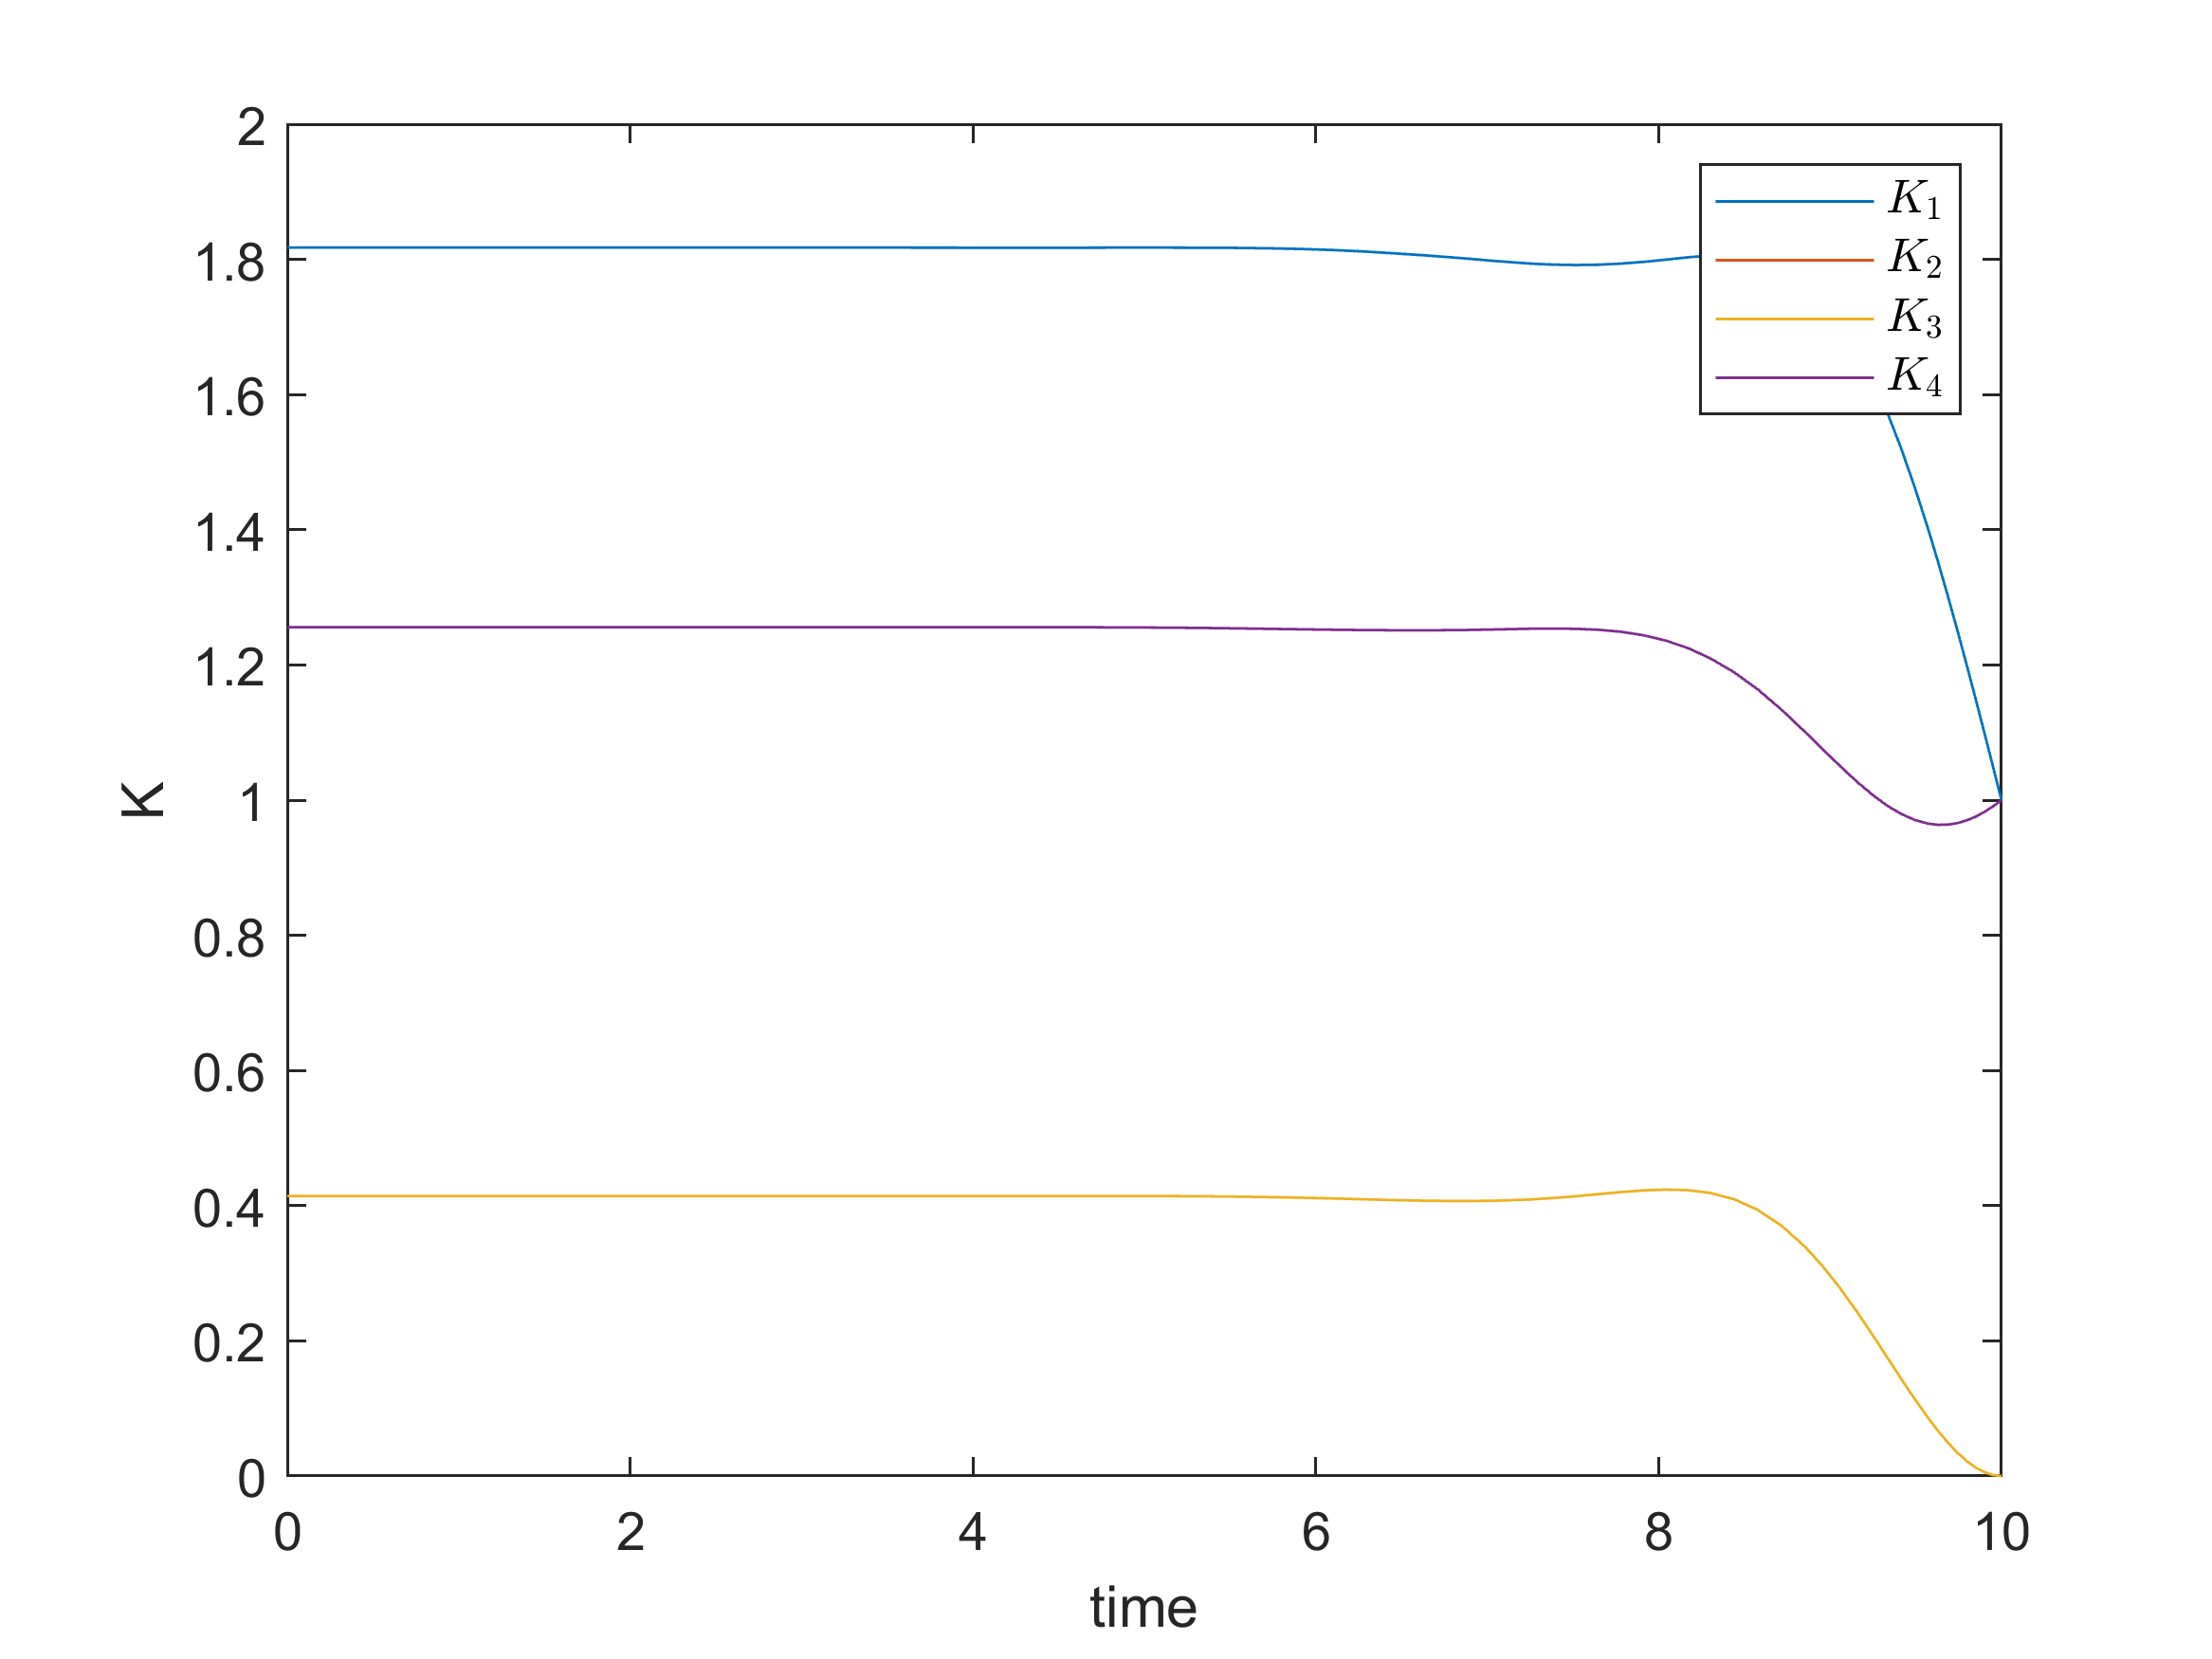
\includegraphics[width=12cm]{../Code/Q3/figures/K10.png}
\end{figure}
\begin{figure}[H]
	\caption{$u(t)$ in $t_f = 10\sec$}
	\centering
	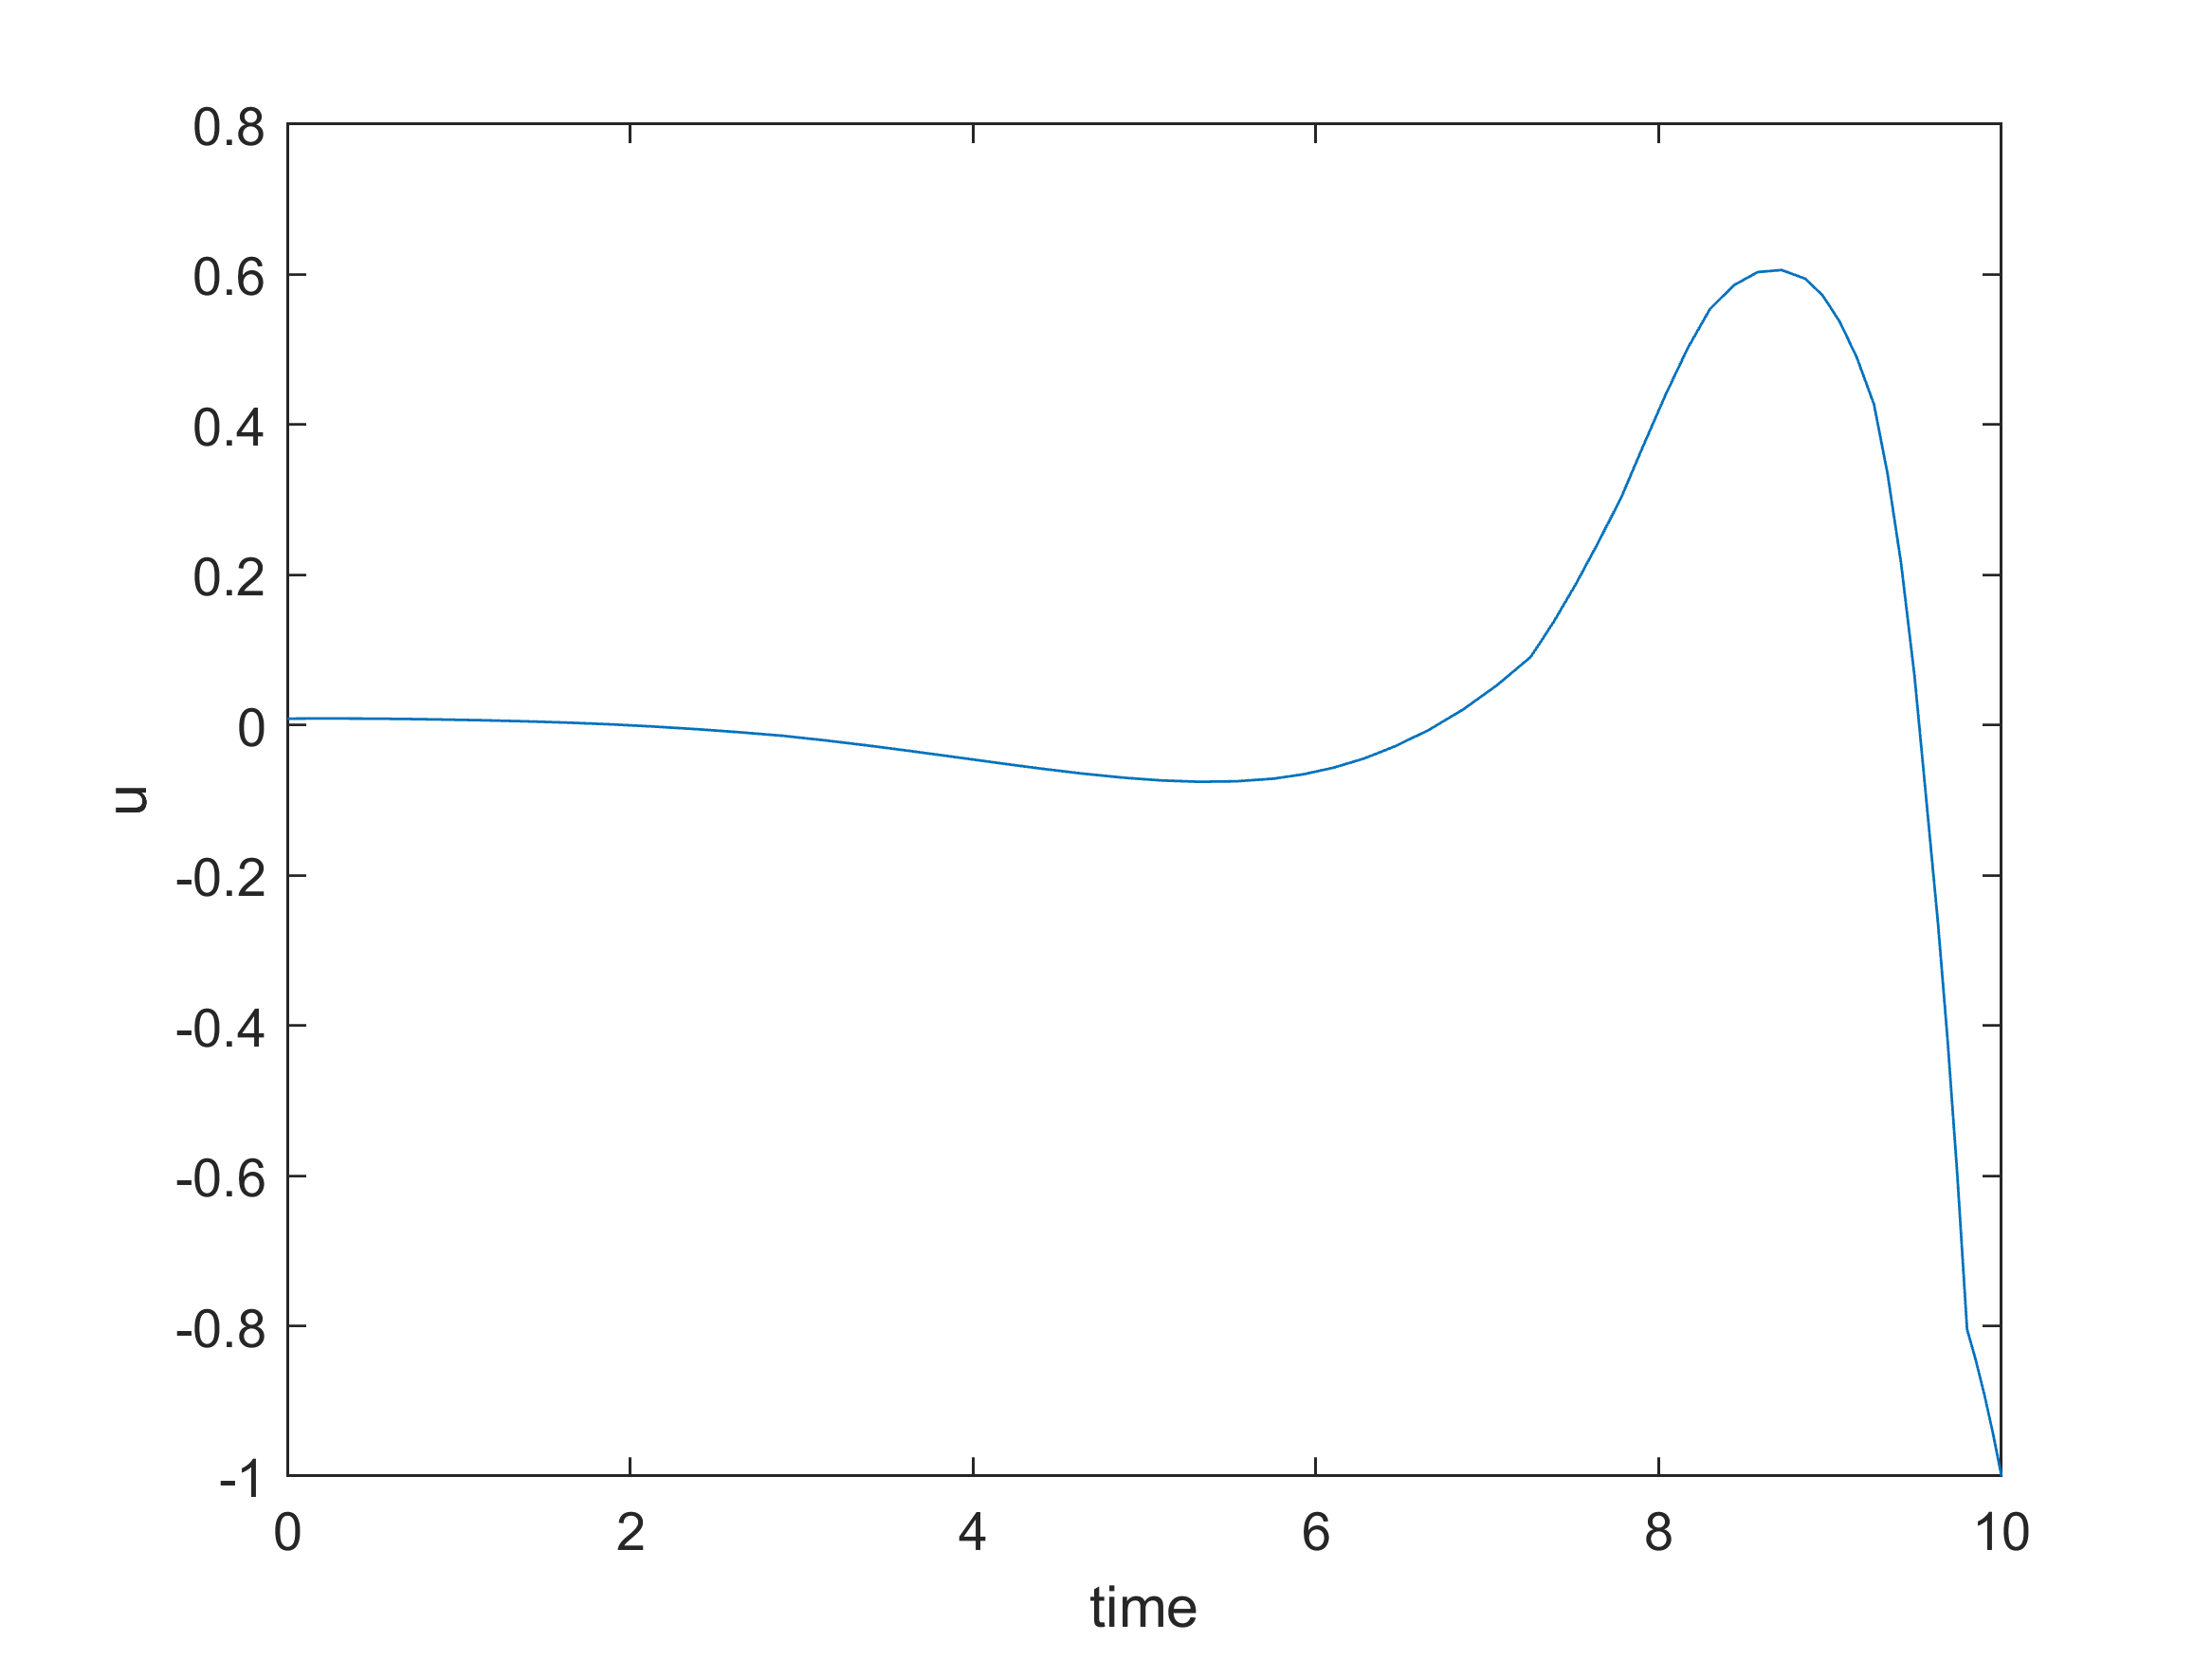
\includegraphics[width=12cm]{../Code/Q3/figures/u10.png}
\end{figure}
\begin{figure}[H]
	\caption{System States $\vec x(t)$ in $t_f = 10\sec$}
	\centering
	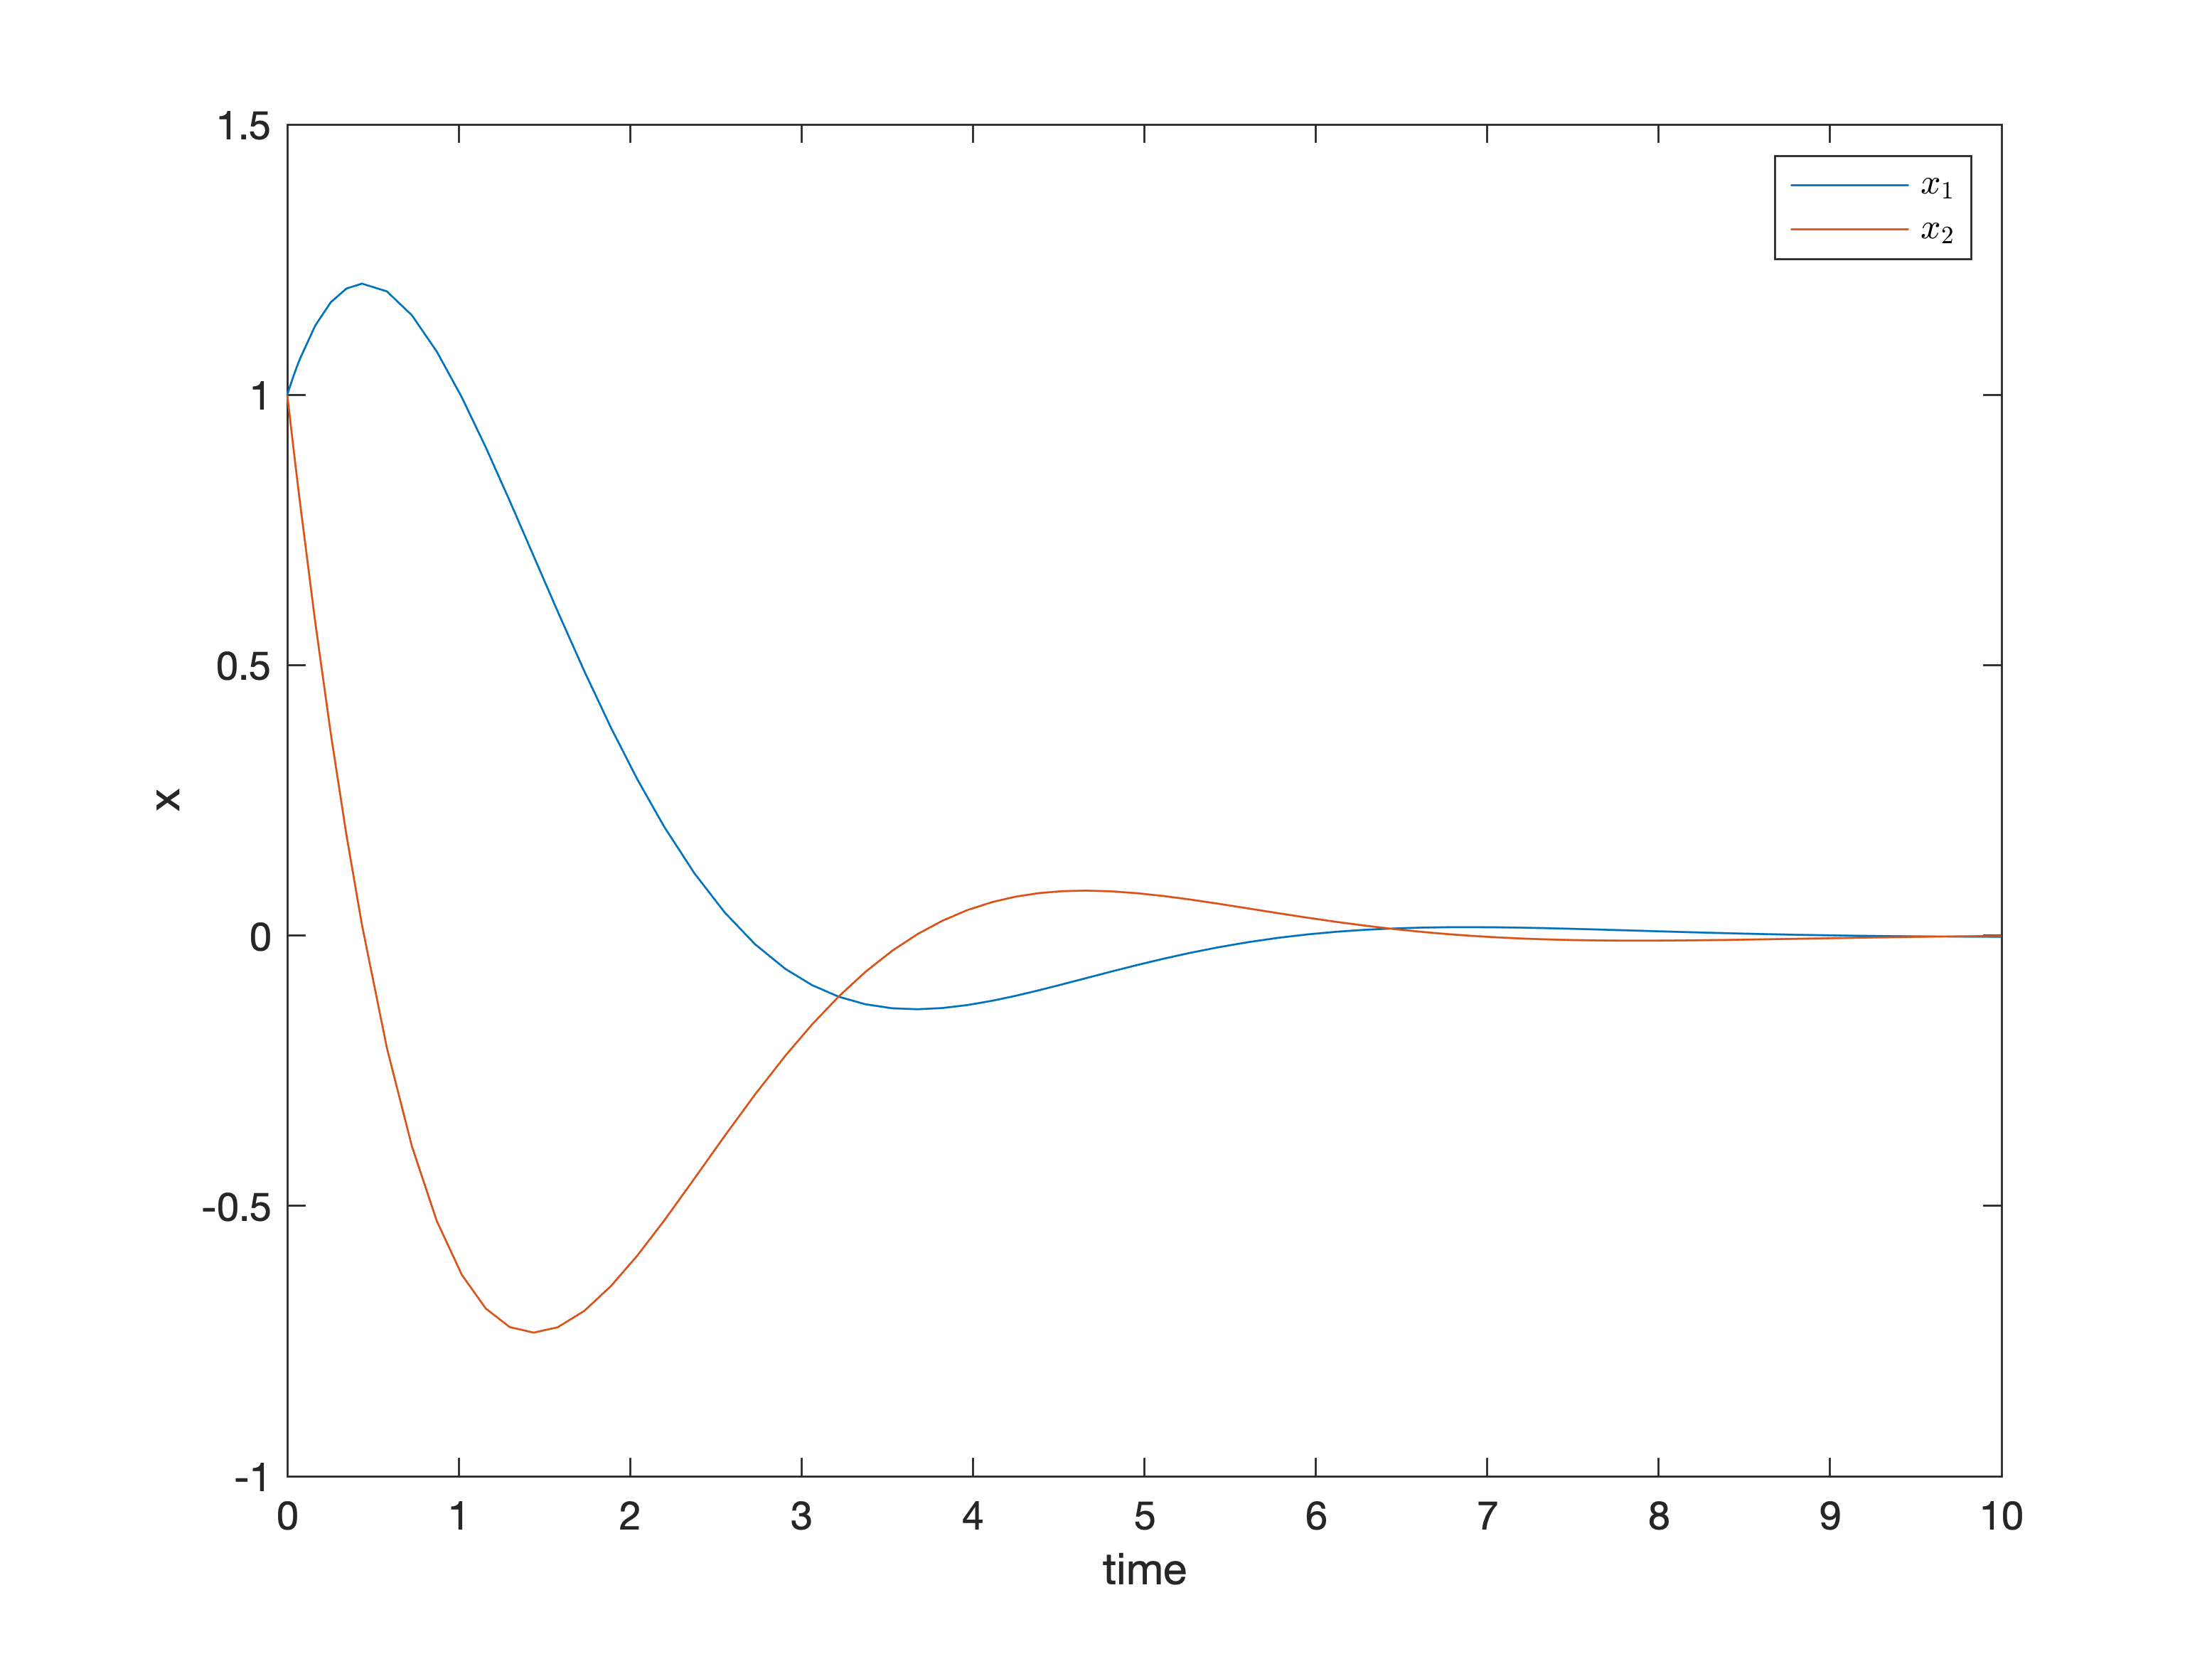
\includegraphics[width=12cm]{../Code/Q3/figures/tf10.png}
\end{figure}
%%%%%%%%% tf = 15 %%%%%%%%%
\item $t_f = 15\sec$
\begin{figure}[H]
	\caption{$K(t)$ in $t_f = 15\sec$}
	\centering
	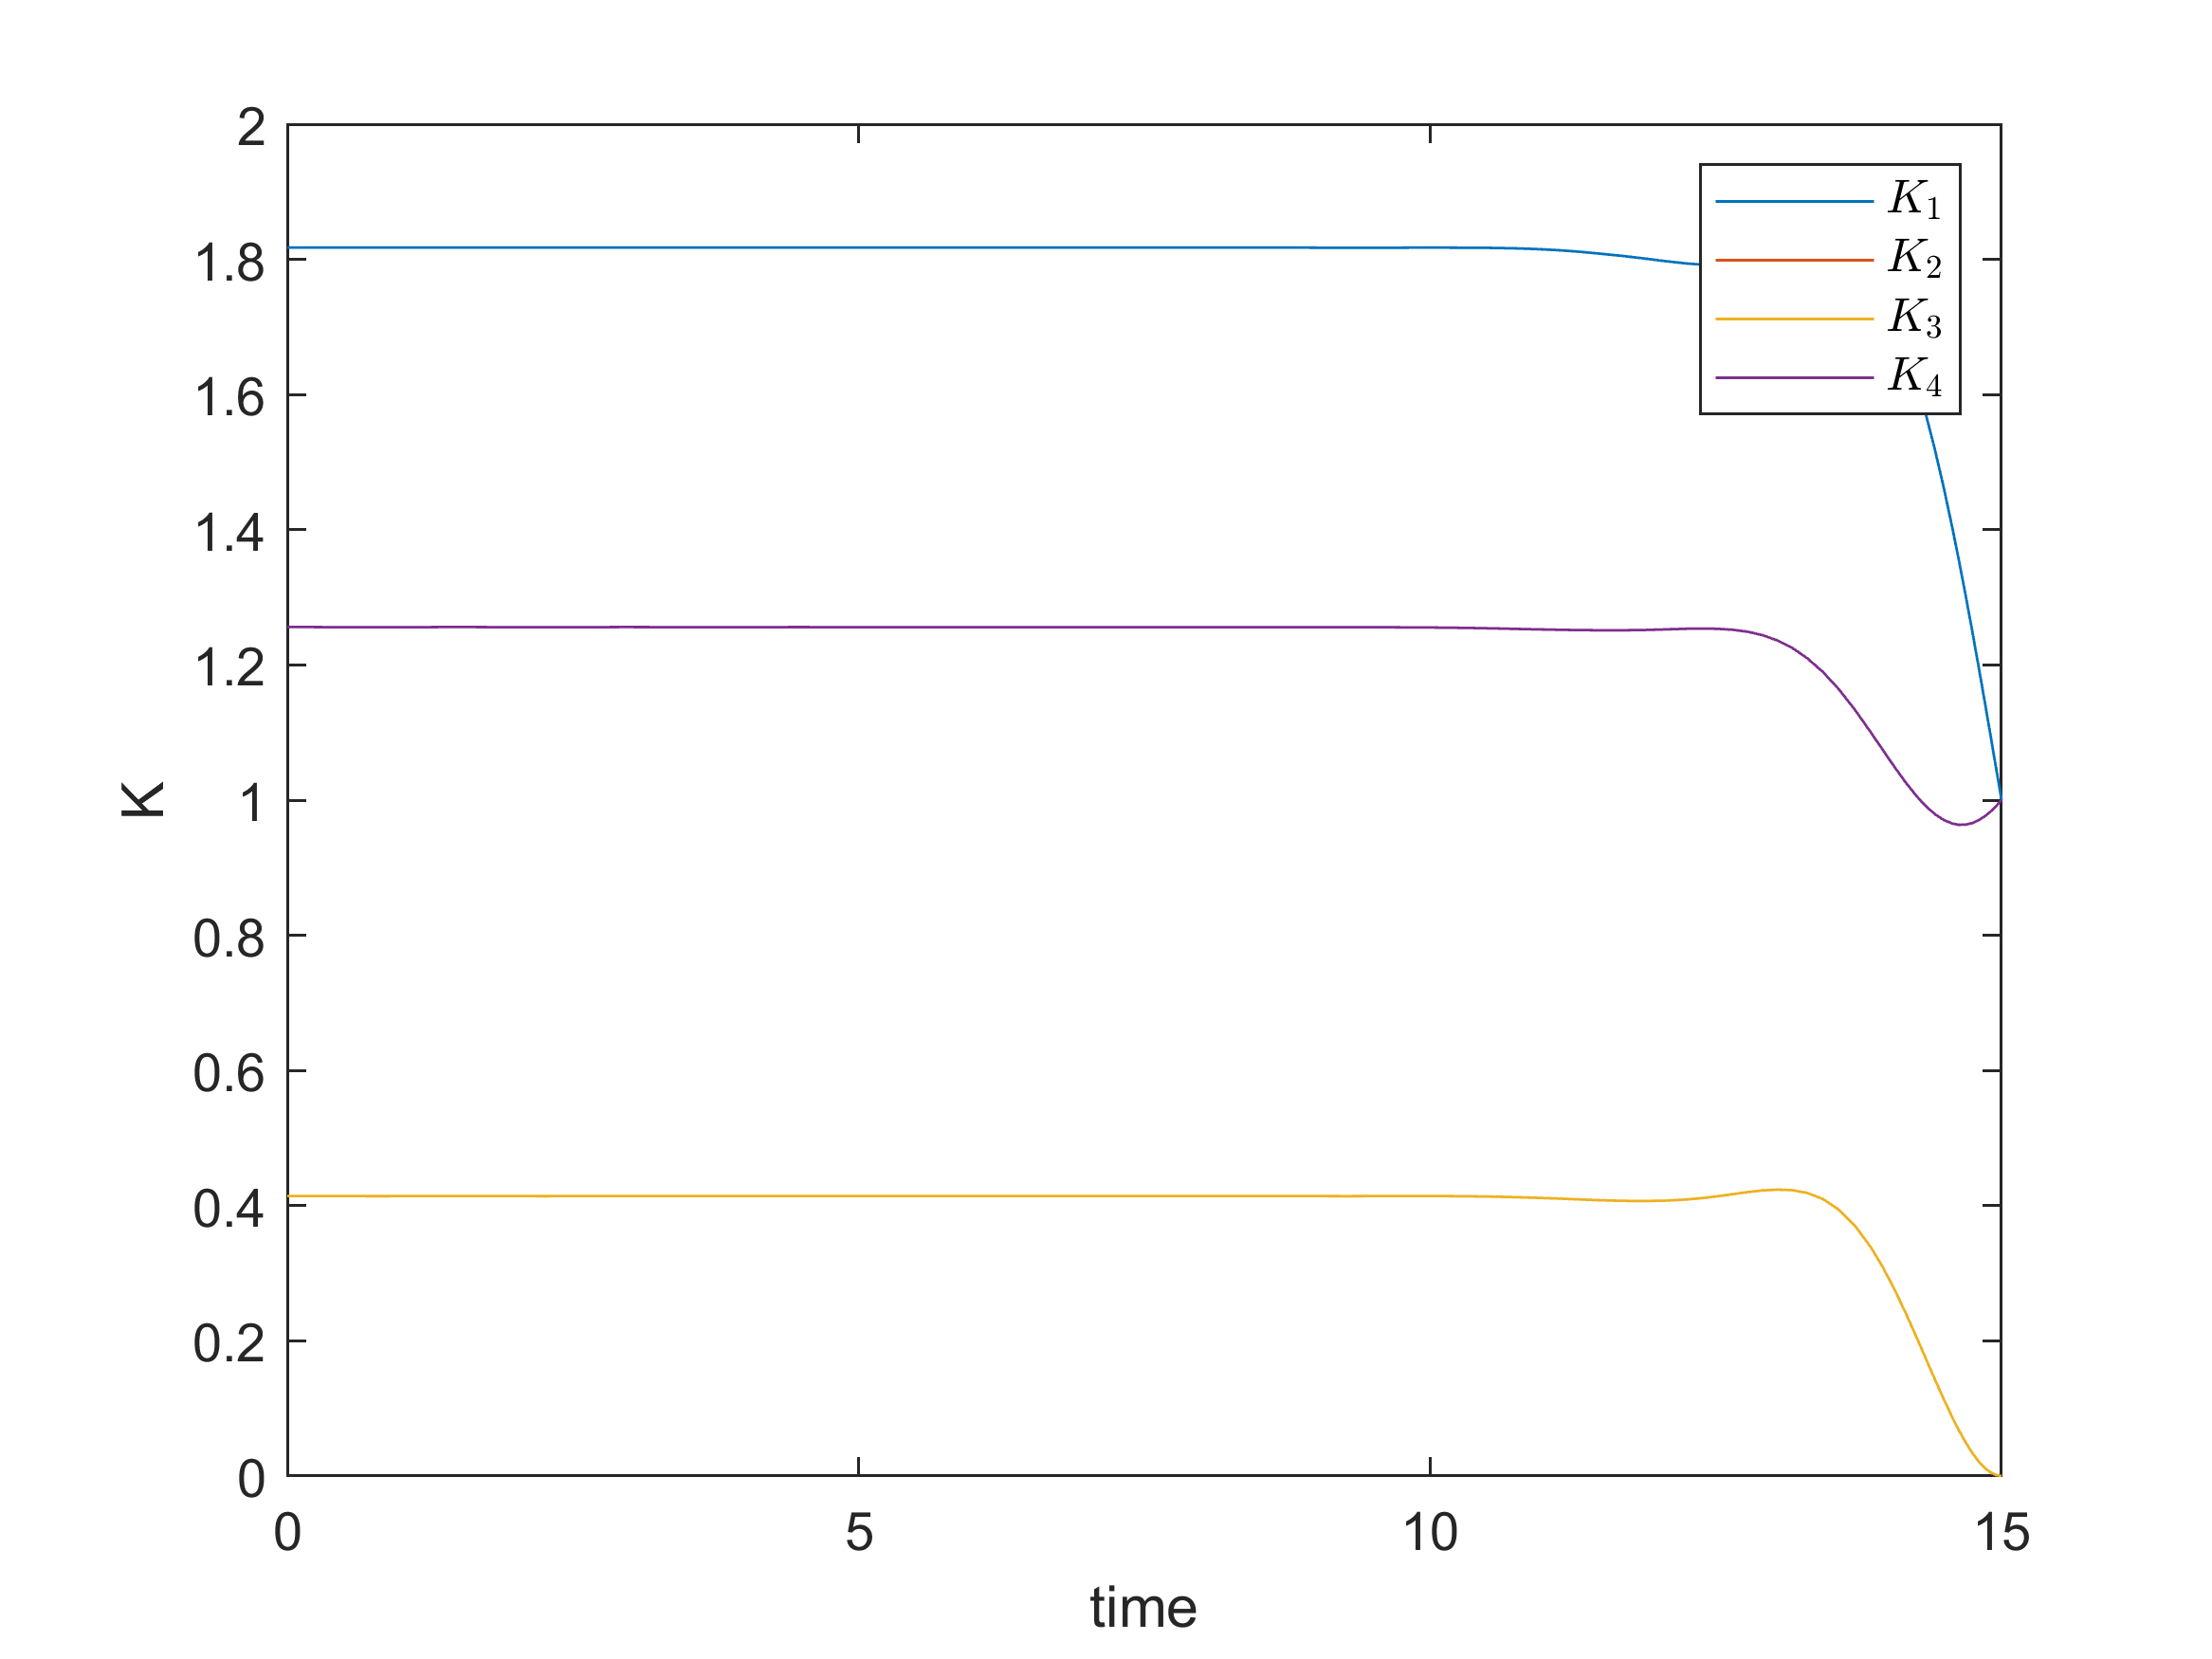
\includegraphics[width=12cm]{../Code/Q3/figures/K15.png}
\end{figure}
\begin{figure}[H]
	\caption{$u(t)$ in $t_f = 15\sec$}
	\centering
	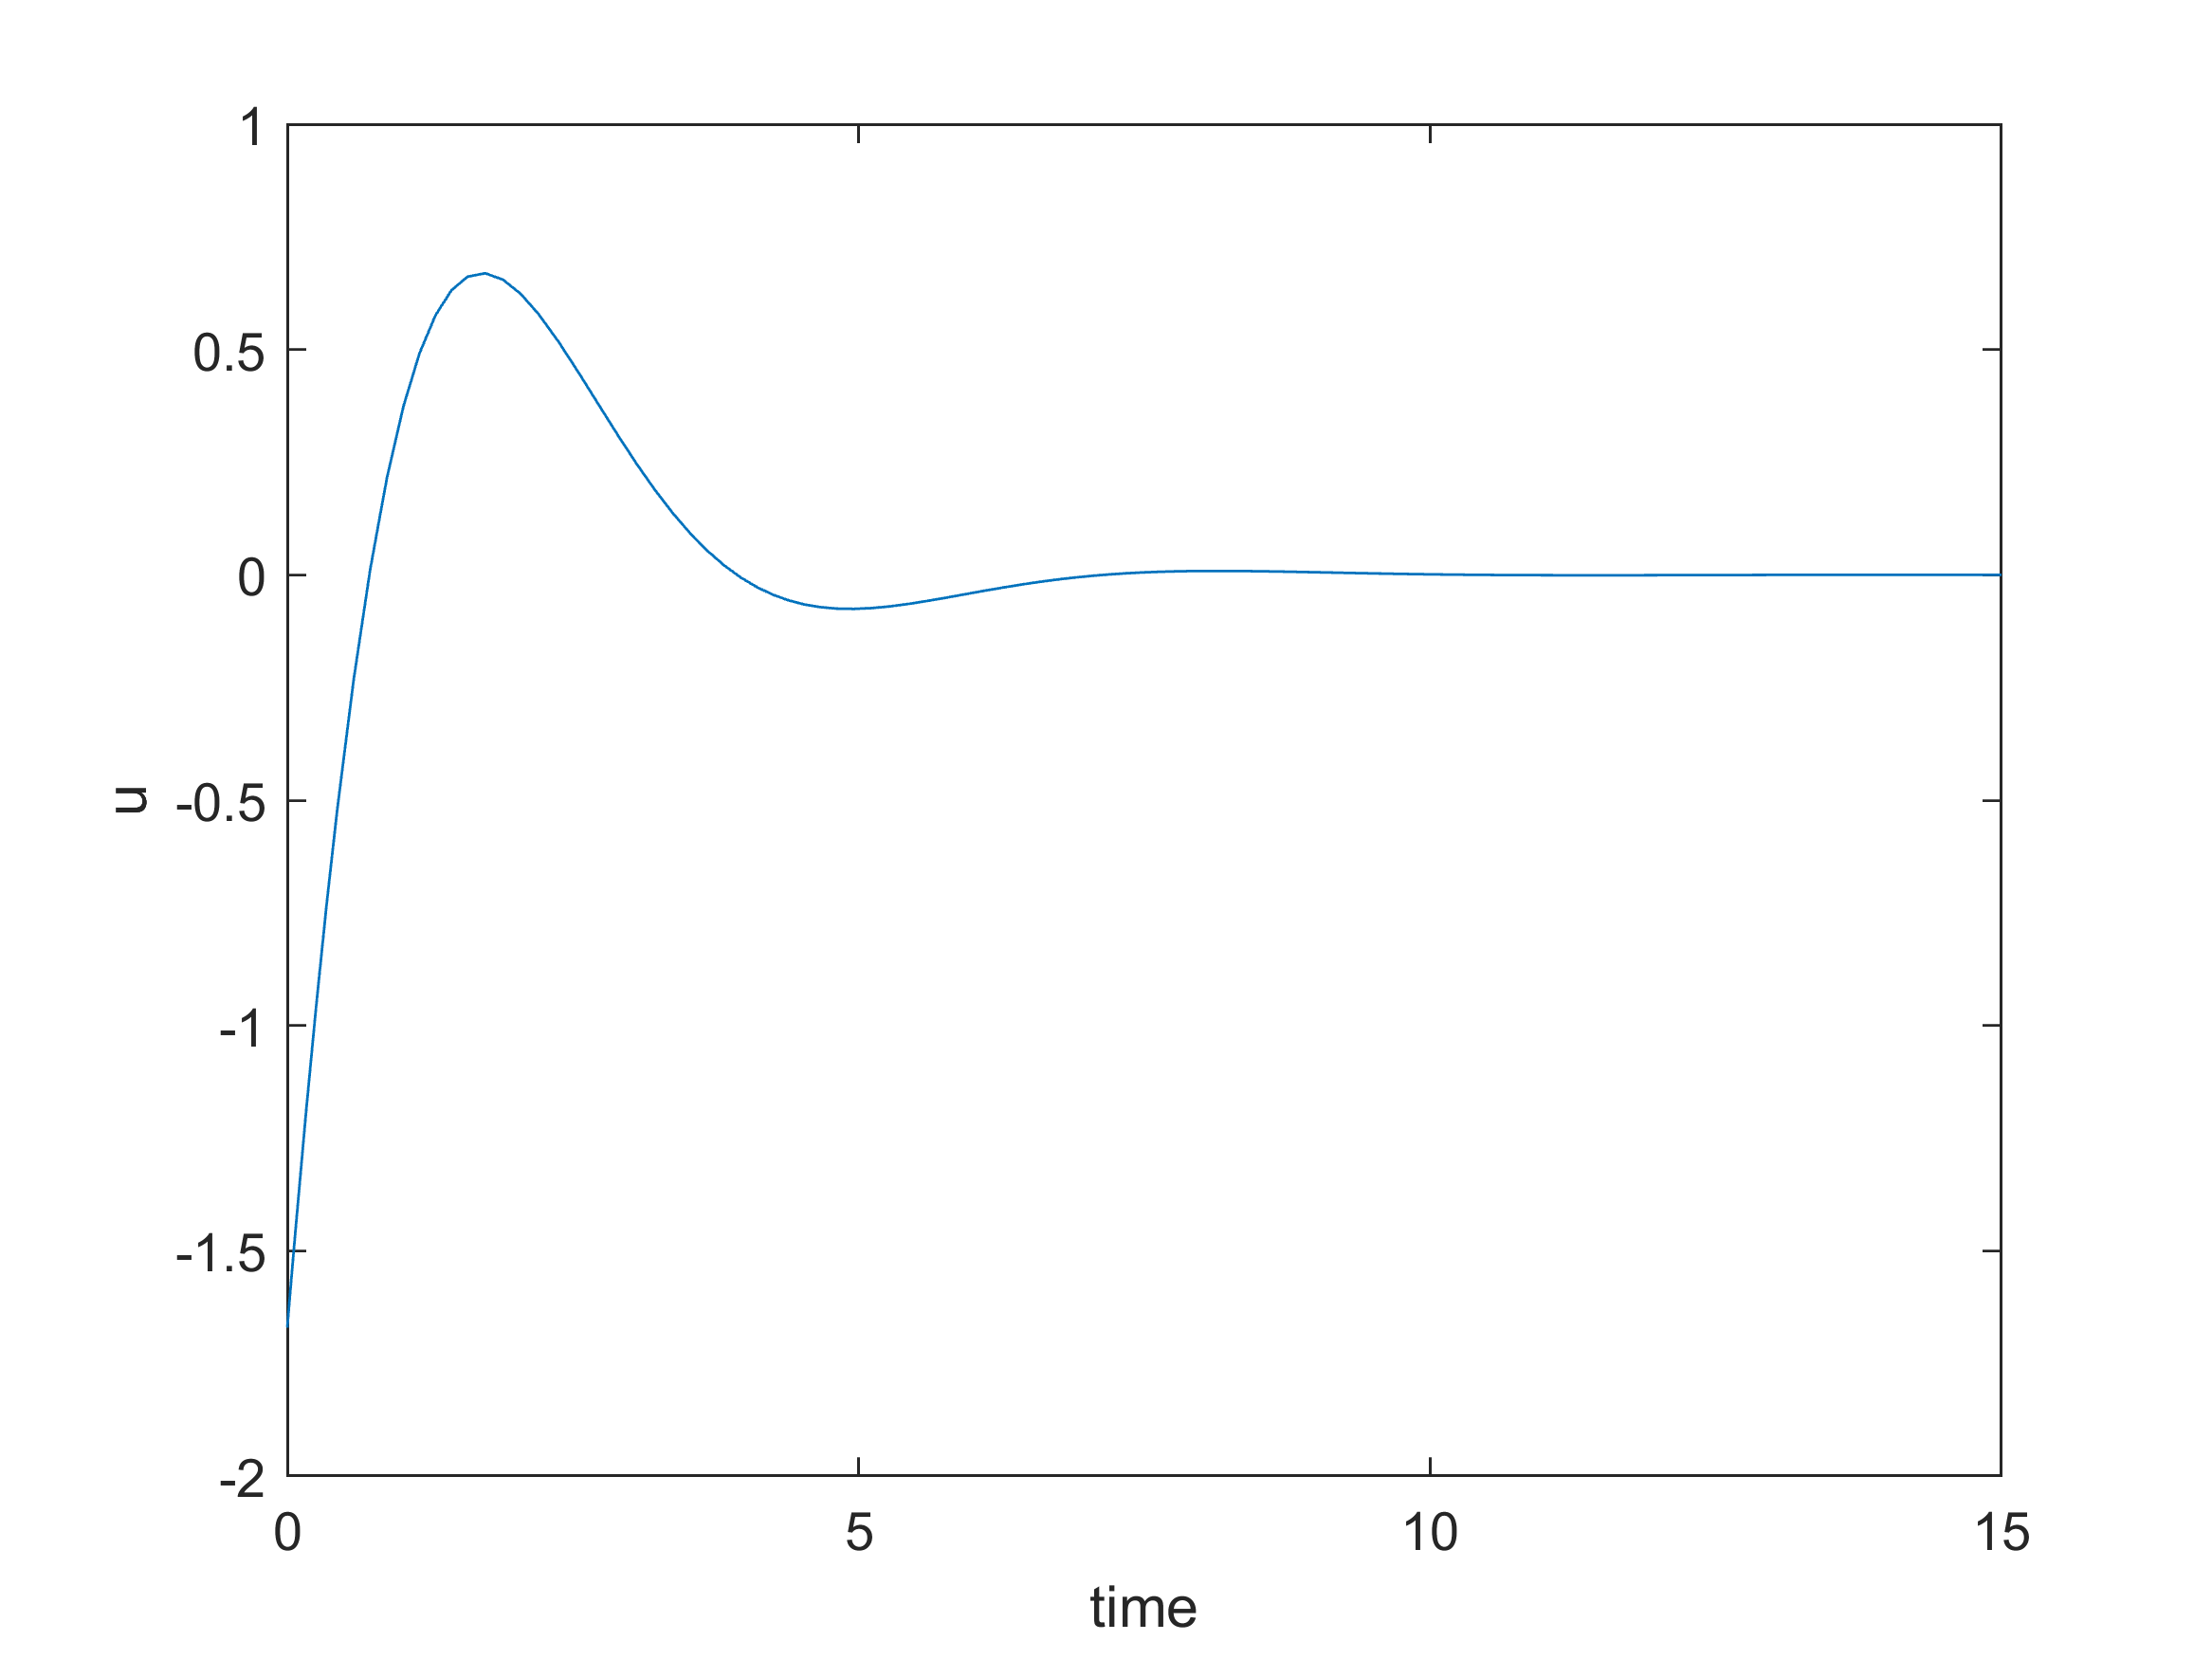
\includegraphics[width=12cm]{../Code/Q3/figures/u15.png}
\end{figure}
\begin{figure}[H]
	\caption{System States $\vec x(t)$ in $t_f = 15\sec$}
	\centering
	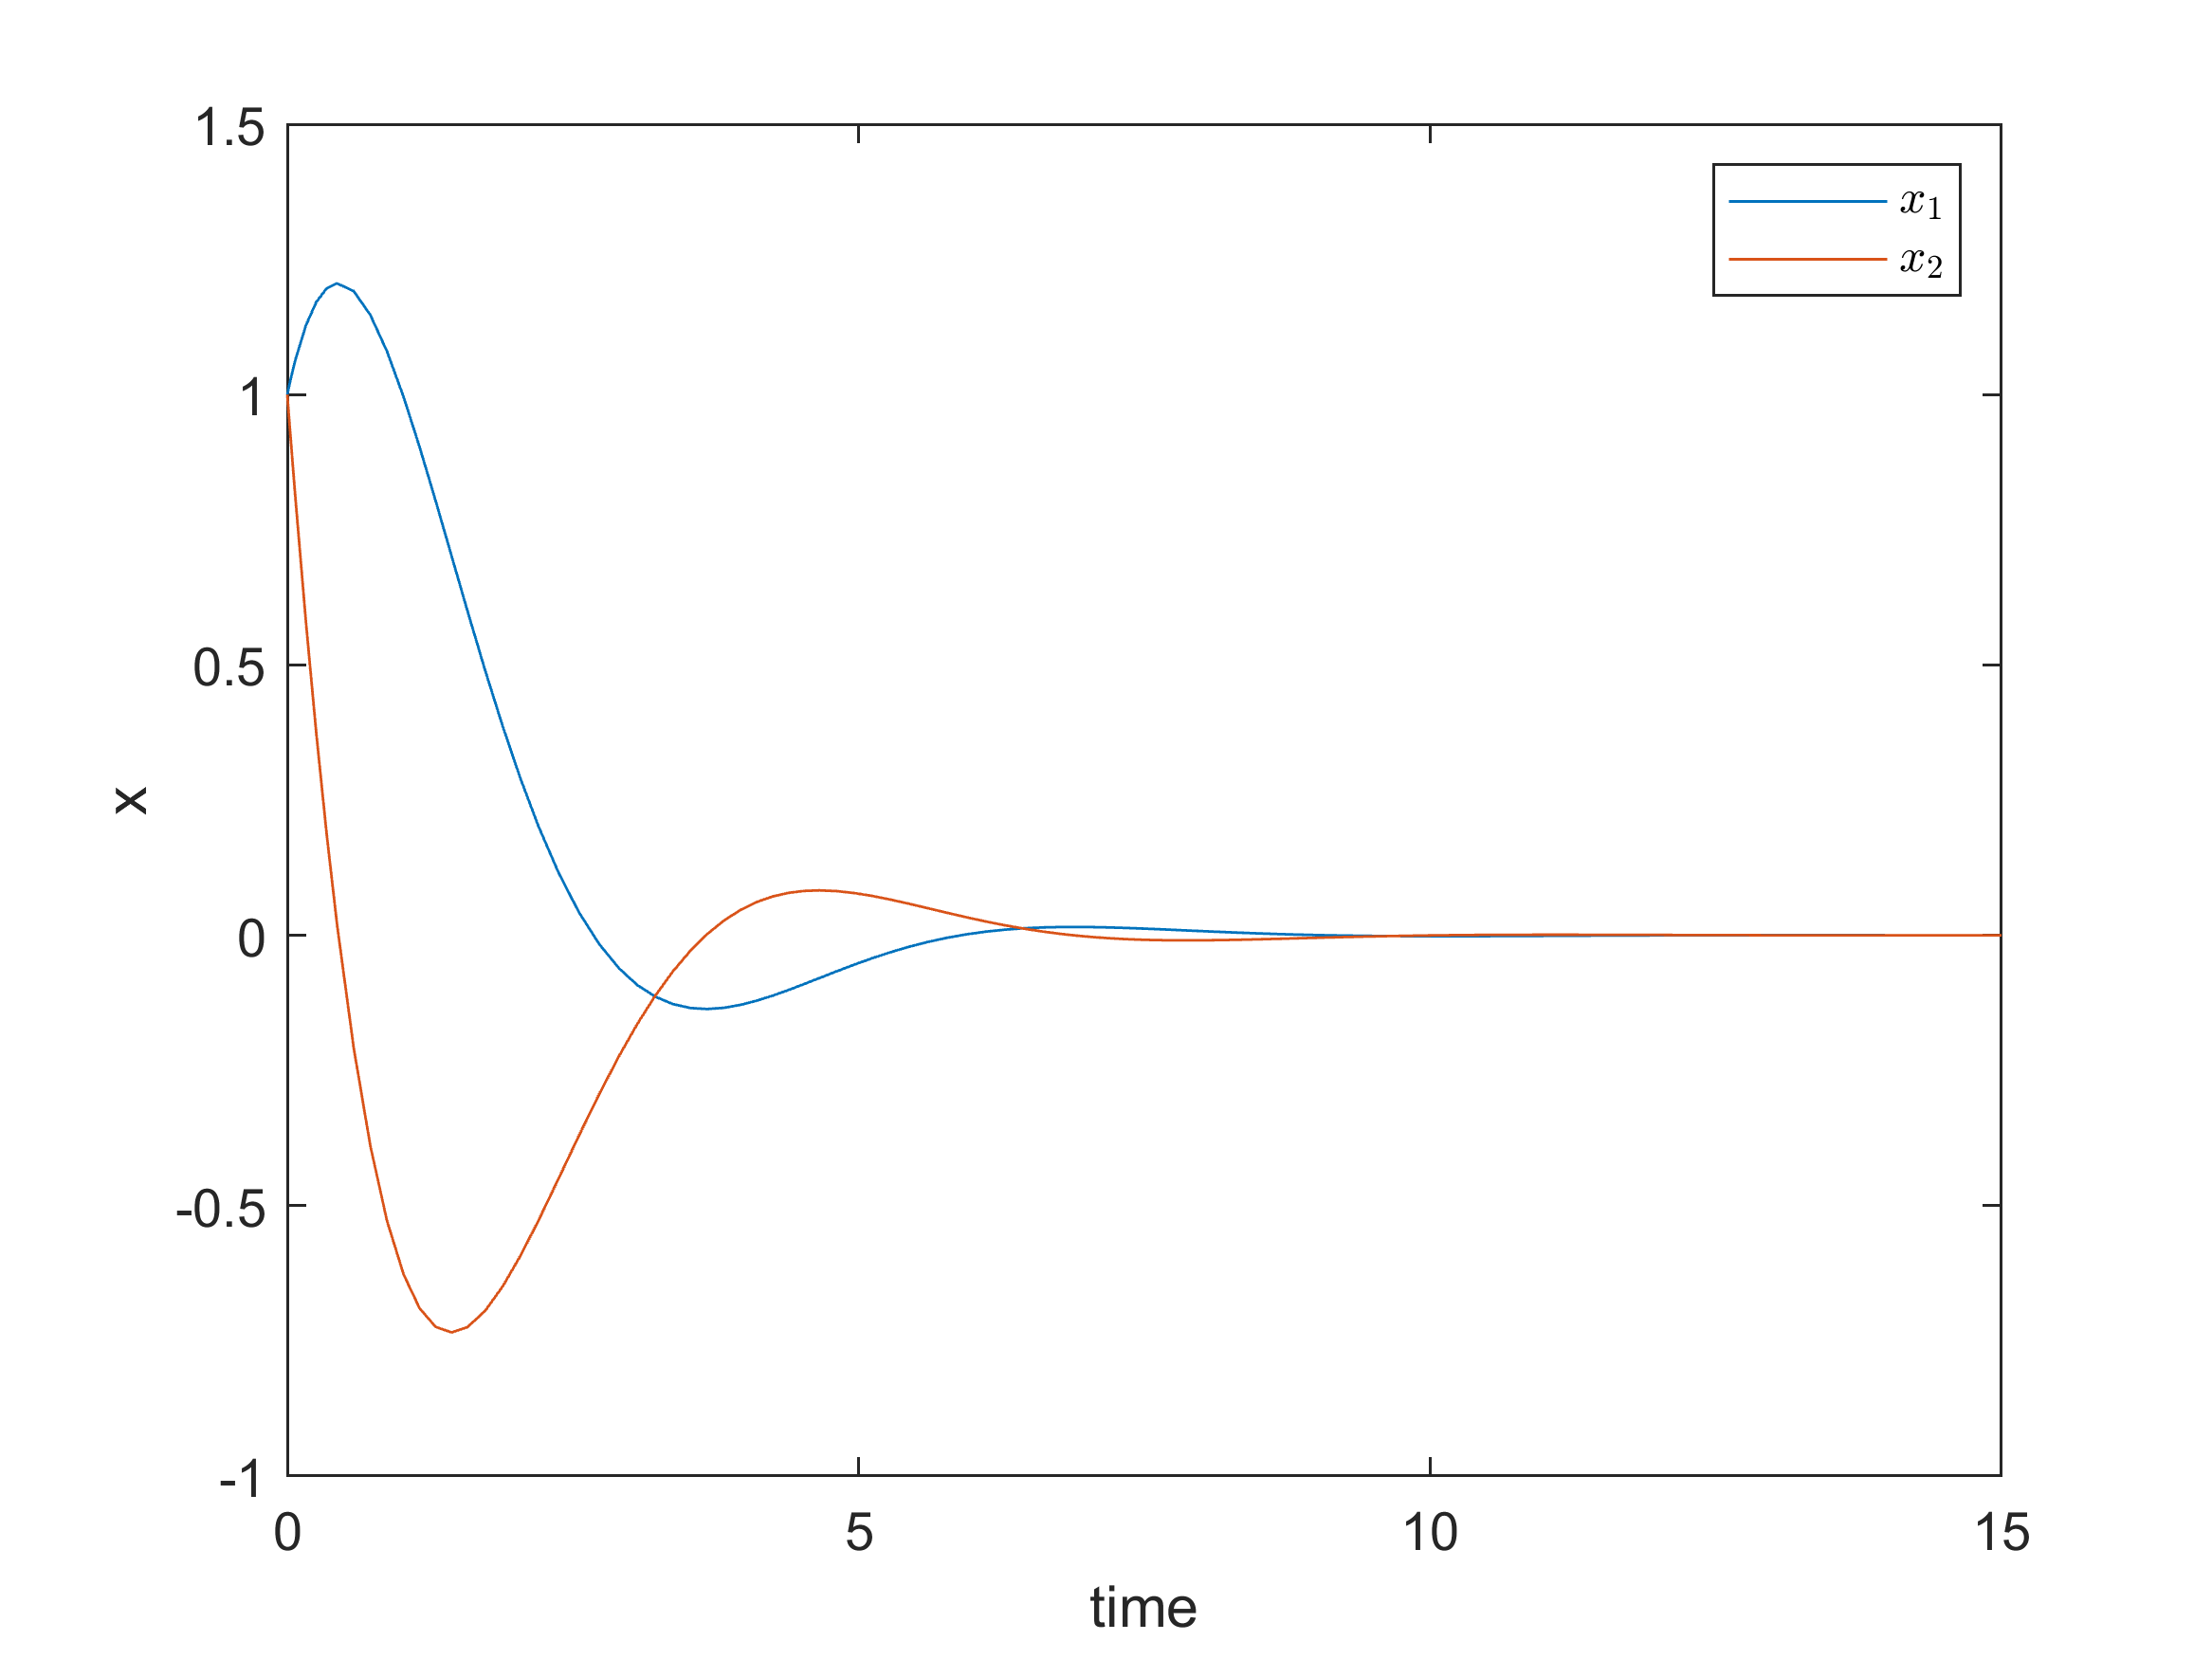
\includegraphics[width=12cm]{../Code/Q3/figures/tf15.png}
\end{figure}
%%%%%%%%% K(t) sub plot %%%%%%%%%
\item $K(t)$ for all simulated $t_f$
\begin{figure}[H]
	\caption{$K(t)$ for all simulated $t_f$}
	\centering
	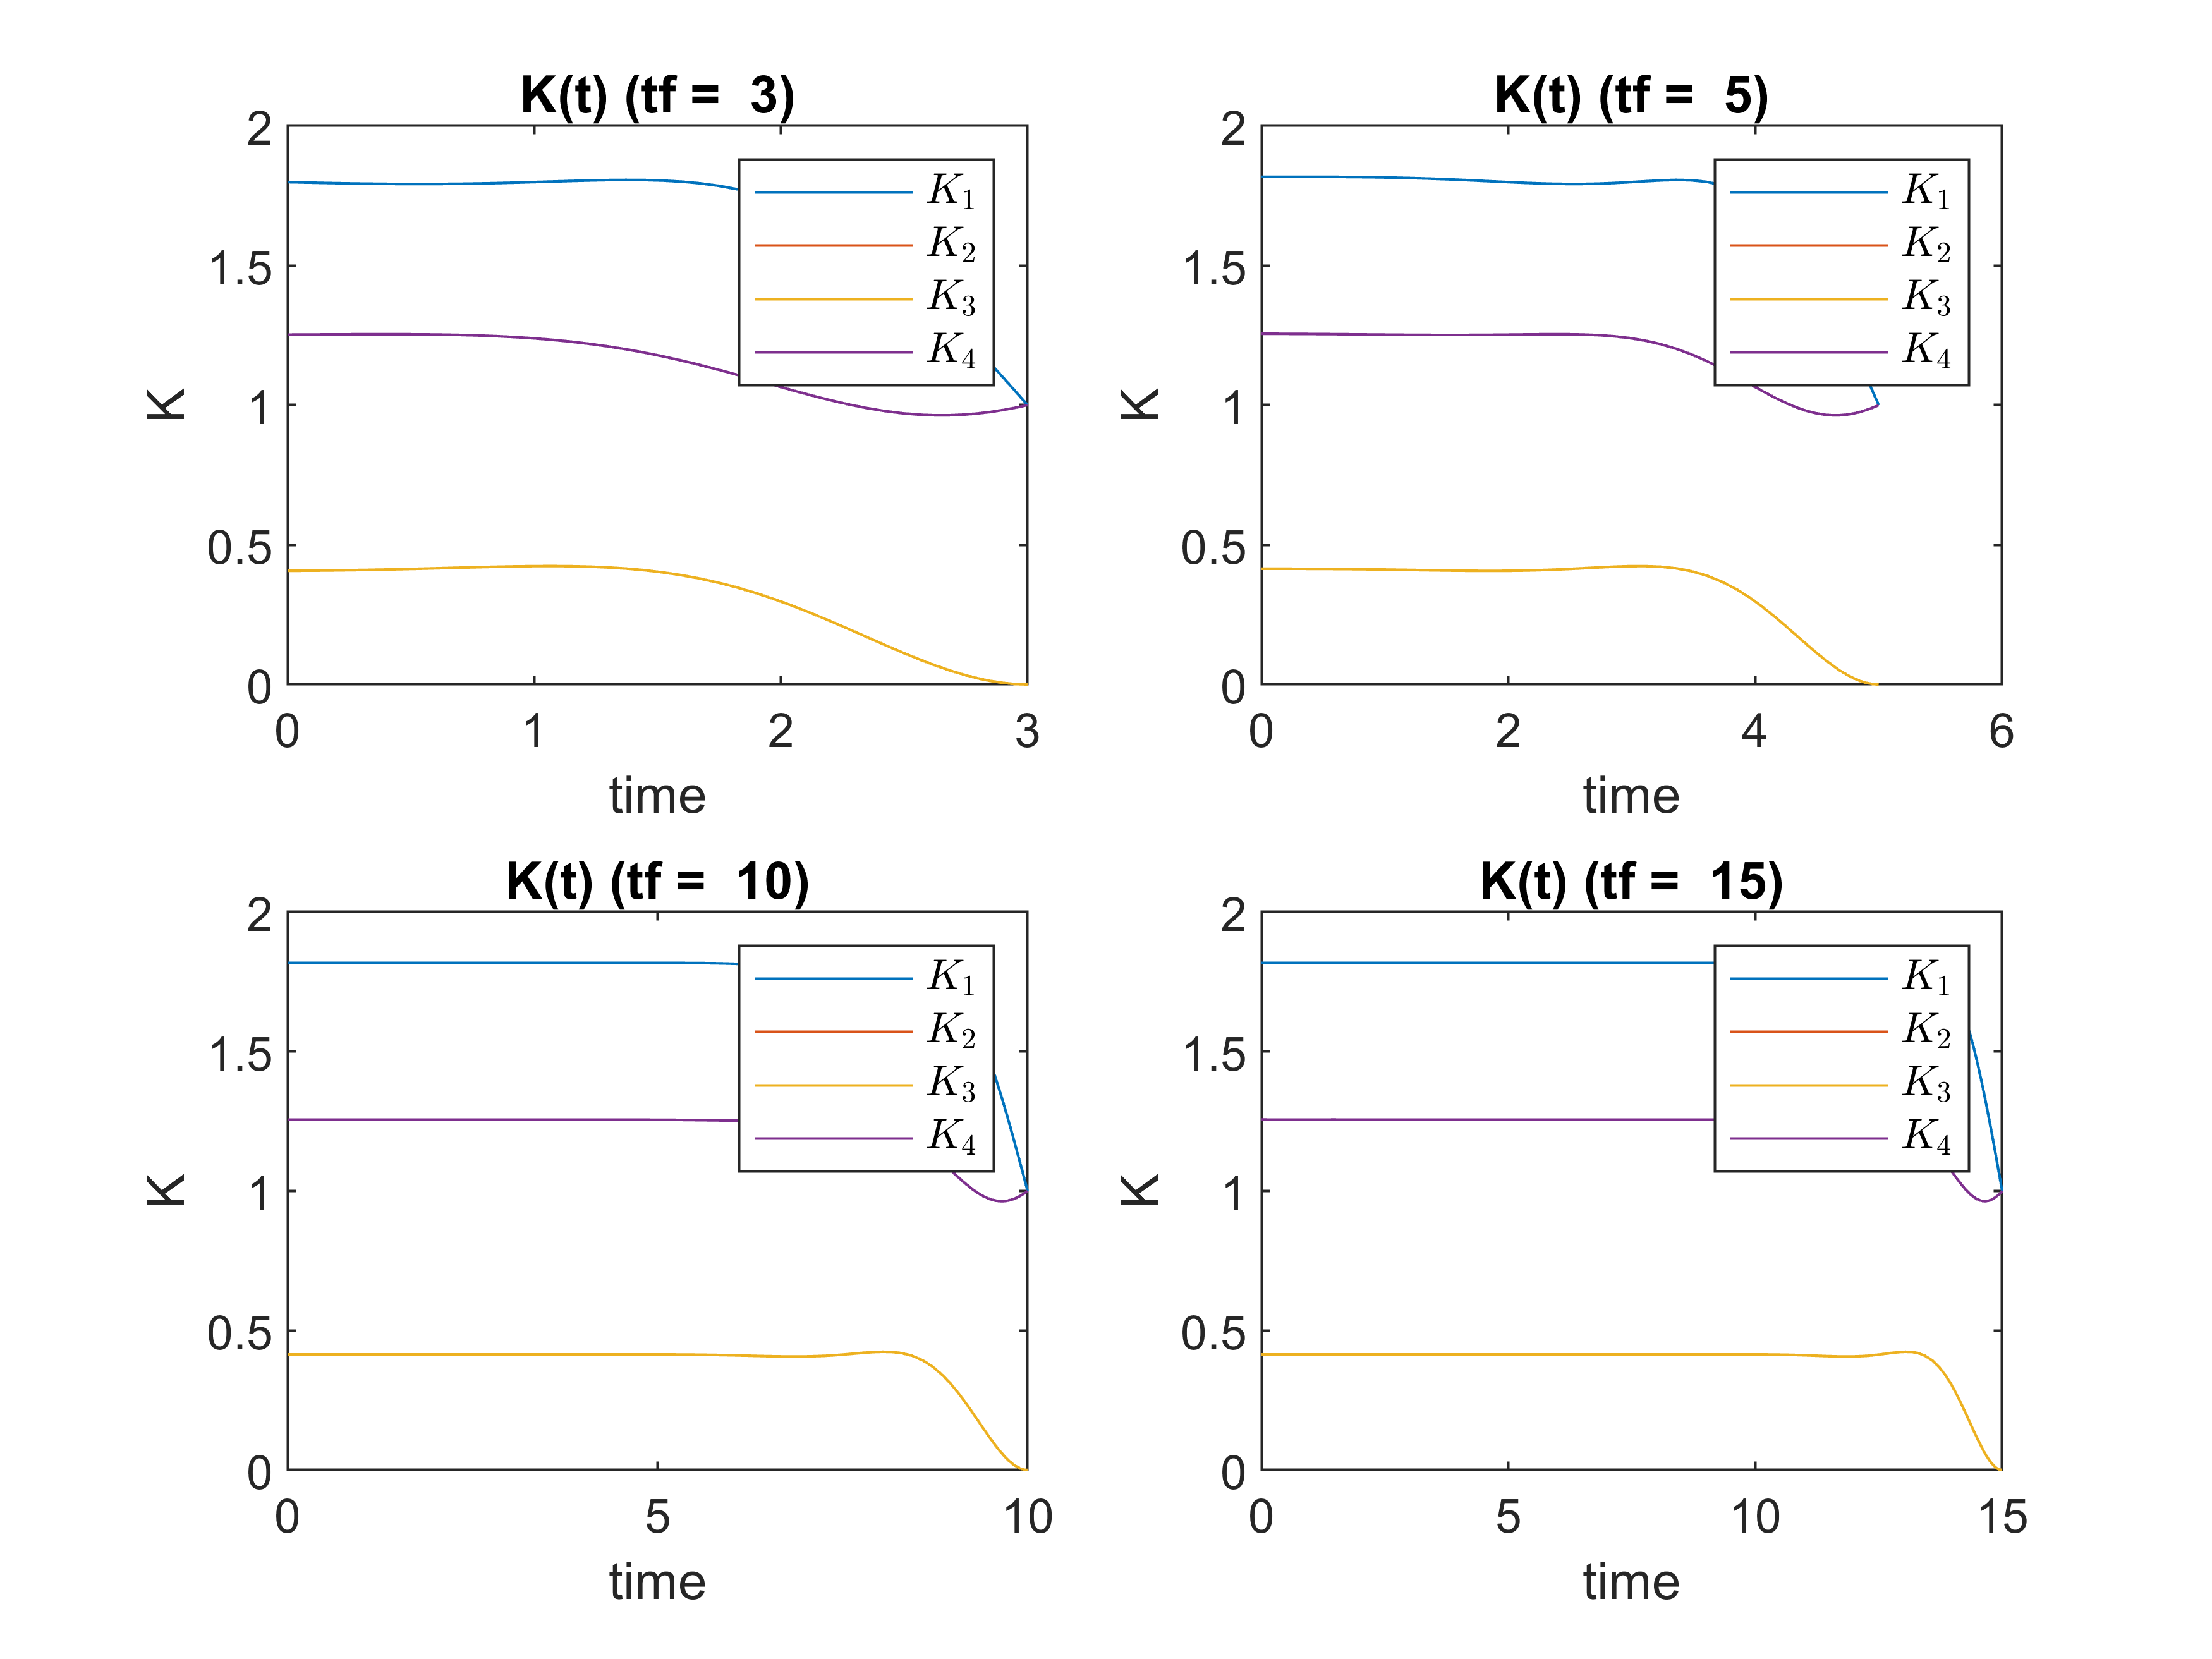
\includegraphics[width=12cm]{../Code/Q3/figures/SubplotQ3_cKI.png}
\end{figure}
%%%%%%%%% u(t) sub plot %%%%%%%%%
\item $u(t)$ for all simulated $t_f$
\begin{figure}[H]
	\caption{$u(t)$ for all simulated $t_f$}
	\centering
	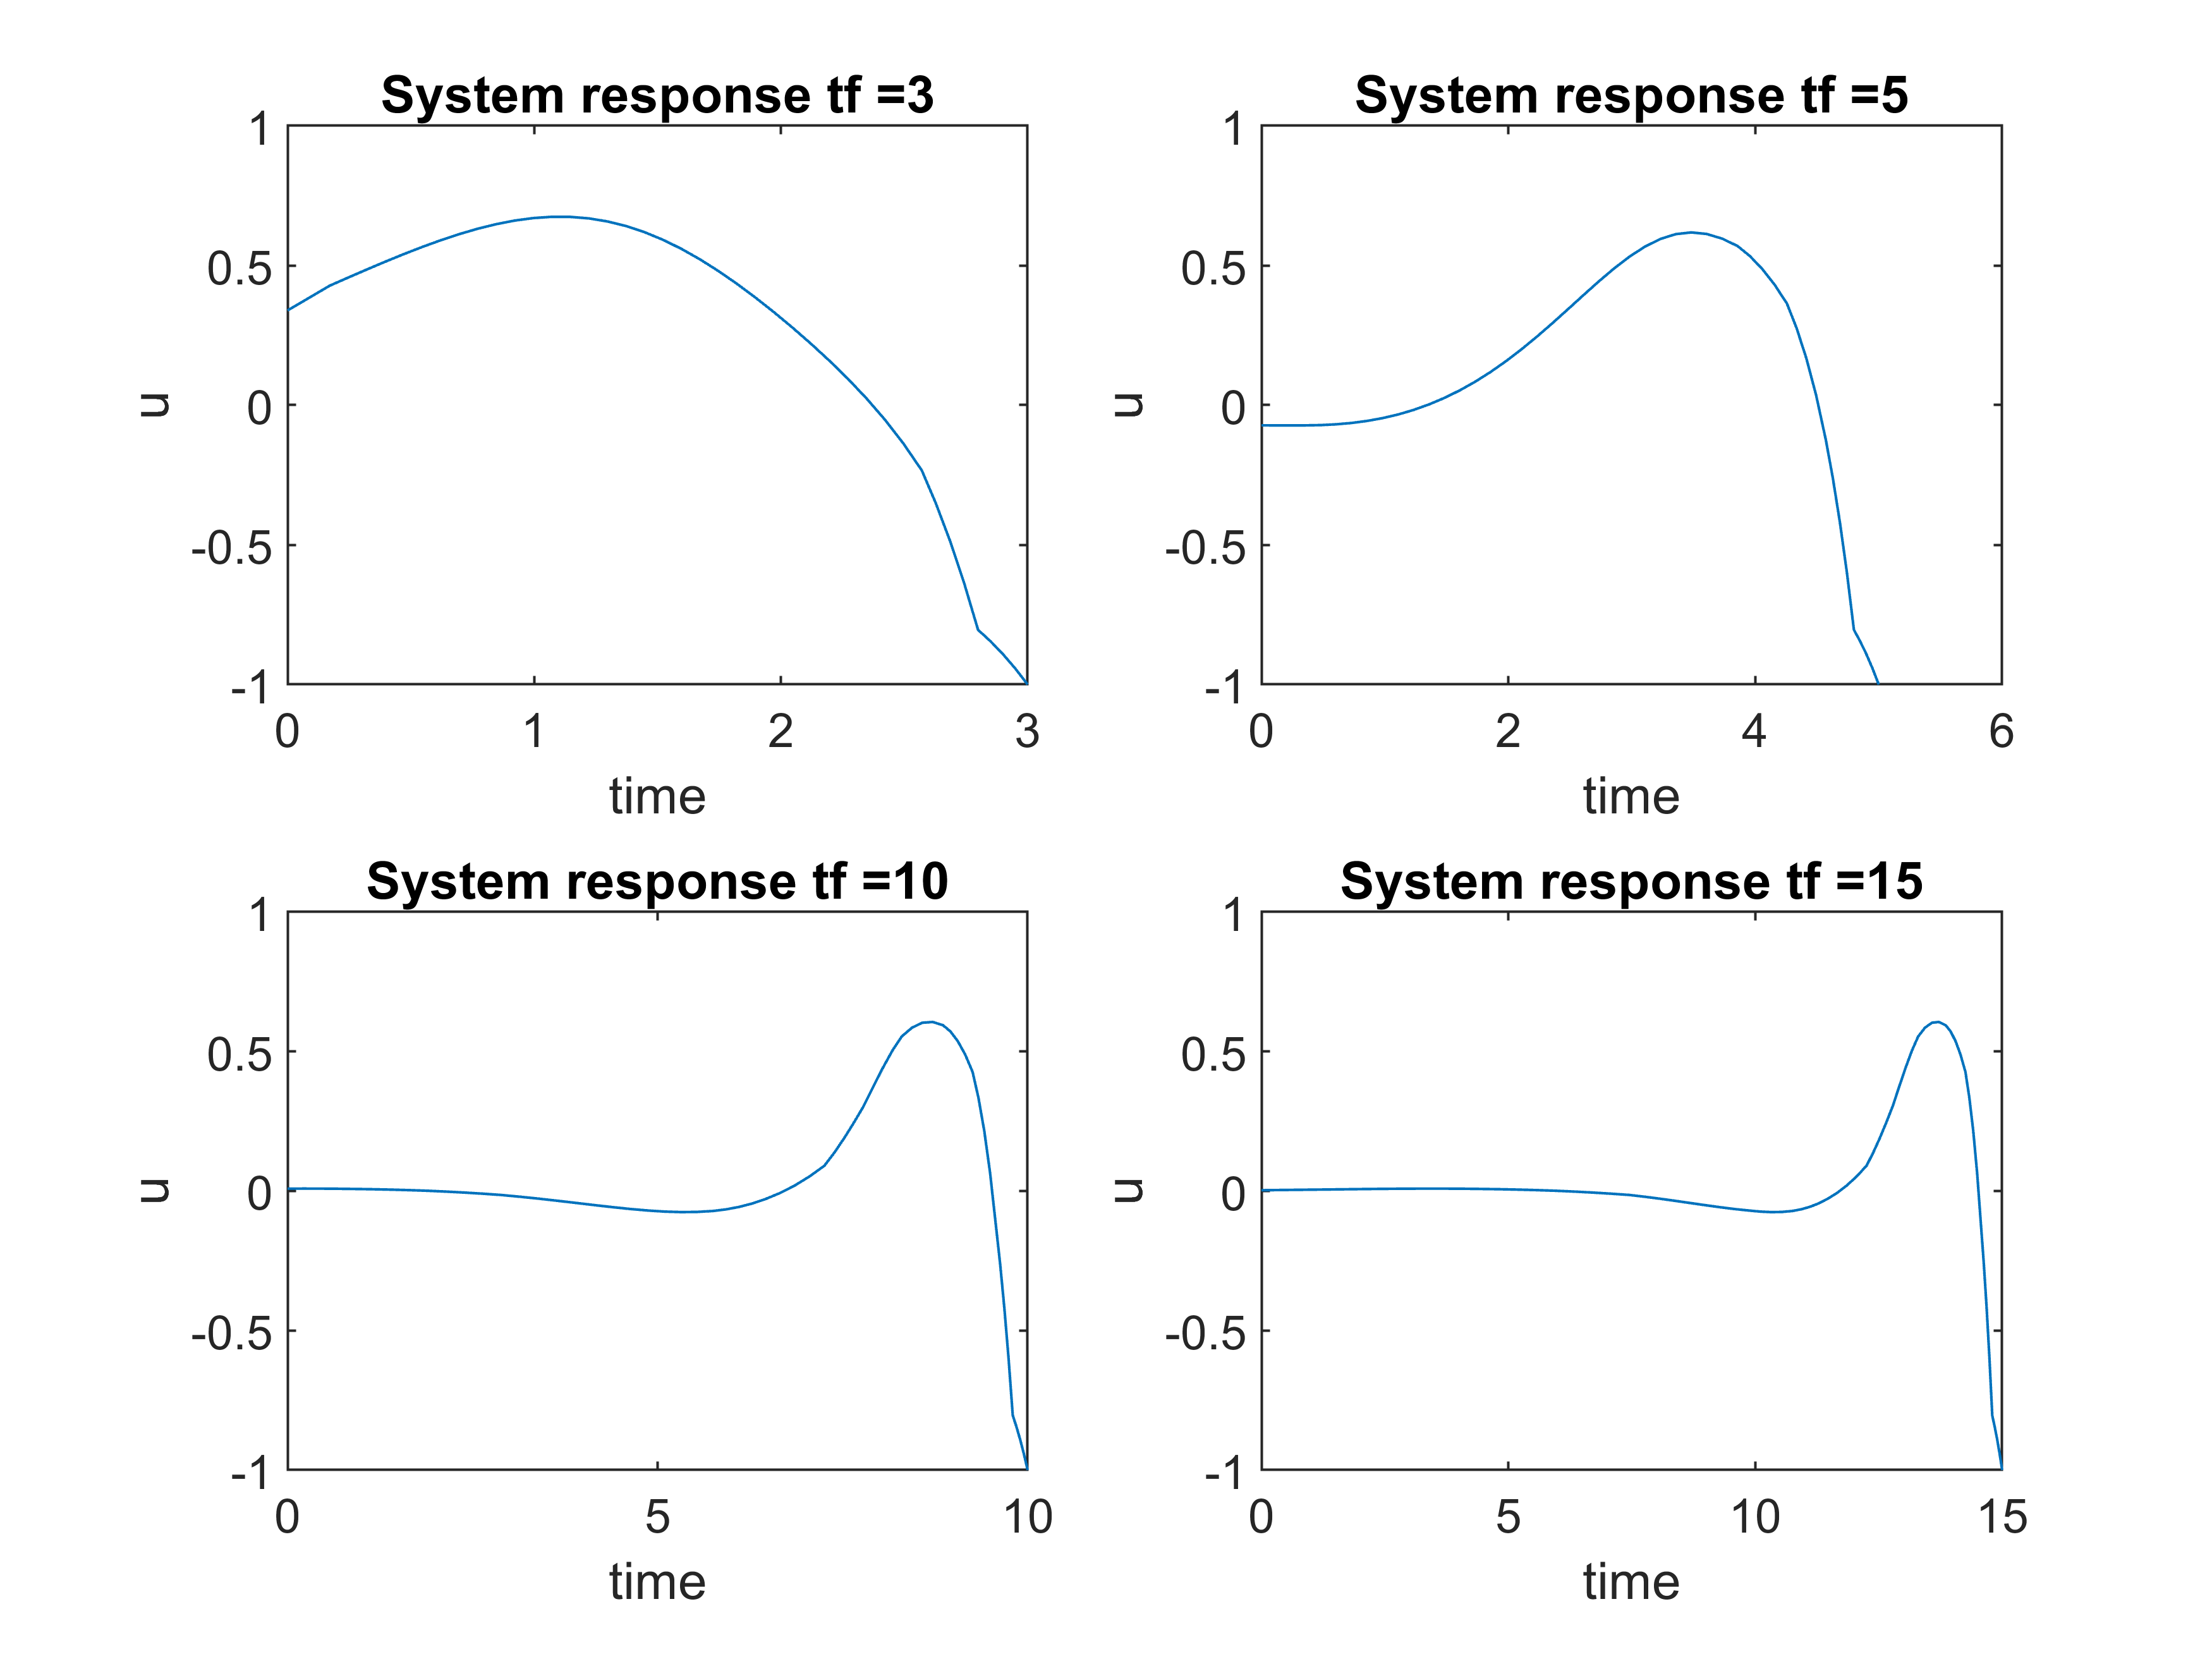
\includegraphics[width=12cm]{../Code/Q3/figures/SubplotQ3_cuI.png}
\end{figure}
%%%%%%%%% x(t) sub plot %%%%%%%%%
\item System States $\vec x(t)$ for all simulated $t_f$
\begin{figure}[H]
	\caption{System States $\vec x(t)$ for all simulated $t_f$}
	\centering
	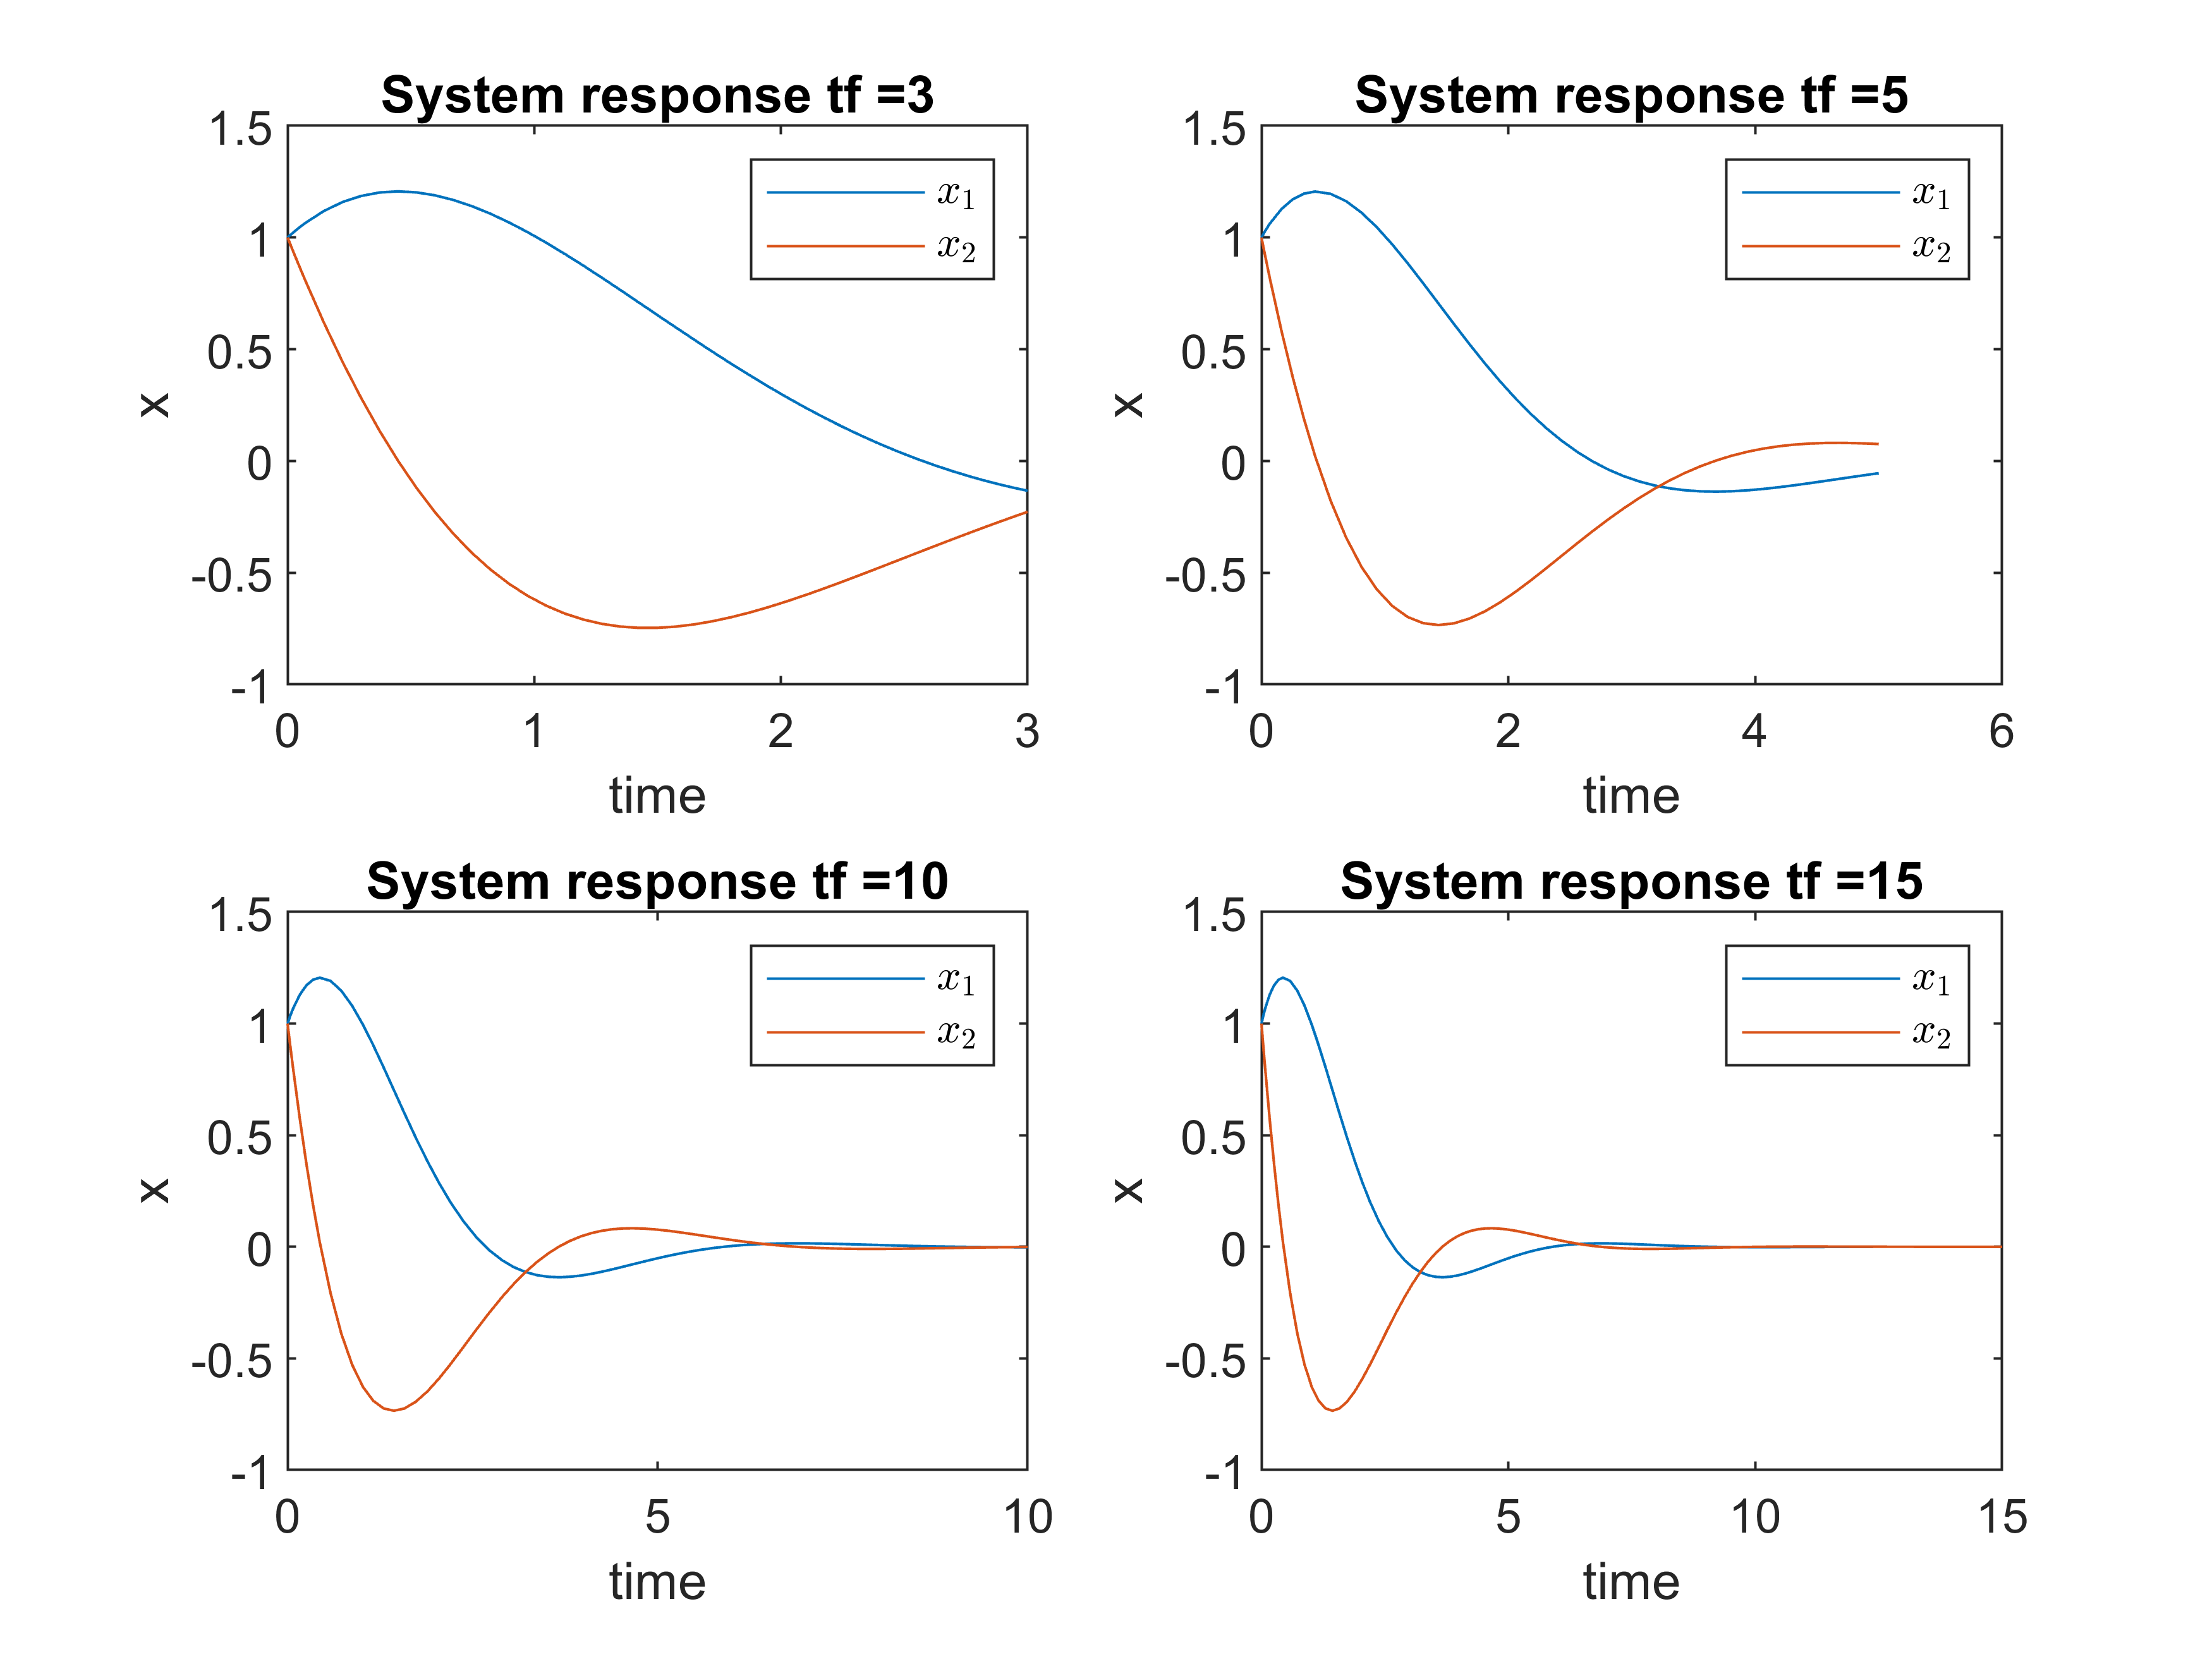
\includegraphics[width=12cm]{../Code/Q3/figures/SubplotQ3_cI.png}
\end{figure}
\end{itemize}
For different times and constant $\alpha, \beta, H$ the trajectory is very similar but in longer time system is more neat to target and of curse use much more energy.